\documentclass{article}

% Conditional compilation.
% NOTE: If you set fullversionfalse, just compile ONCE so that TOC stays unchanged.
\newif\iffullversion
\fullversiontrue
%\fullversionfalse


%%%%%%%%%%%%%%%%%%%%%%%%%%%%%%%%%%%%%%%%%%%%%%%%%%%%%%%%%%%%%%%%%%%%%%%%%
\pagestyle{plain}                                                      %%
%%%%%%%%%% EXACT 1in MARGINS %%%%%%%                                   %%
\setlength{\textwidth}{6.5in}     %%                                   %%
\setlength{\oddsidemargin}{0in}   %% (It is recommended that you       %%
\setlength{\evensidemargin}{0in}  %%  not change these parameters,     %%
\setlength{\textheight}{8.5in}    %%  at the risk of having your       %%
\setlength{\topmargin}{0in}       %%  proposal dismissed on the basis  %%
\setlength{\headheight}{0in}      %%  of incorrect formatting!!!)      %%
\setlength{\headsep}{0in}         %%                                   %%
\setlength{\footskip}{.5in}       %%                                   %%
%%%%%%%%%%%%%%%%%%%%%%%%%%%%%%%%%%%%                                   %%
\newcommand{\required}[1]{\section*{\hfil #1\hfil}}                    %%
\renewcommand{\refname}{\hfil References Cited\hfil}                   %%
\bibliographystyle{plain}                                              %%
%%%%%%%%%%%%%%%%%%%%%%%%%%%%%%%%%%%%%%%%%%%%%%%%%%%%%%%%%%%%%%%%%%%%%%%%%

\usepackage{graphicx}
\usepackage{color}

\pagestyle{empty}


\usepackage{fancyvrb}

\newenvironment{bluecode}{\VerbatimEnvironment \color{blue} \begin{Verbatim}}
{\end{Verbatim}}

\usepackage{makeidx}

\makeindex

\begin{document}

\large

\vbox{}
\begin{figure}[!ht]
%\hspace{-4mm}

\includegraphics[width=8cm]{img/logo.png}
\vspace{18mm}
\end{figure}

\begin{figure}[!ht]
\begin{center}
%\hspace{-4mm}
%\hspace{-20mm}
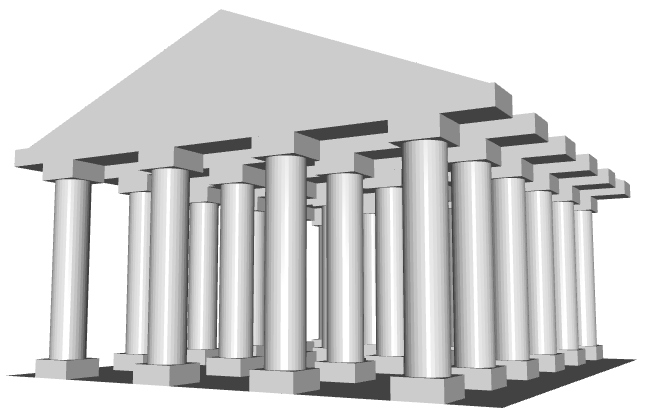
\includegraphics[width=8cm]{img/plasm-temple.png}\hspace{1cm}
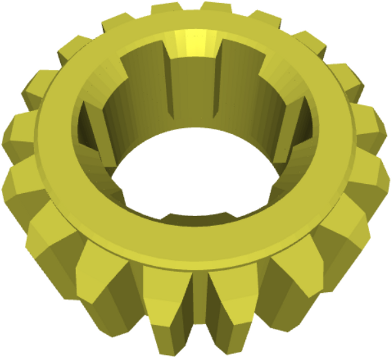
\includegraphics[width=5.5cm]{img/plasm-frontpage.png}
\vspace{15mm}
\end{center}
\end{figure}

\begin{center}
{\Huge \bf Solid Modeling with PLaSM}\\
\vbox{}
\vspace{1.4cm}
\iffullversion
\else
\centerline{\huge \color{red}{PREVIEW}}
\fi
\vfill
{\large
{\bf Pavel Solin \& Alberto Paoluzzi}
}
\end{center}
\vfill
\vfill
\begin{center}
Revision Oct-10-2012. Copyright 2012 FEMhub Inc. All rights reserved.
\end{center}
\newpage

%%%%%%%%%%%%%%%%%%%%%%%%%%%%%%%%%%%%%%%%%%%%%%%%%%%%%%%%%%%%%%%%%%%%%%%%%

\vbox{}
\vfill
{
\noindent
{\bf About this Textbook}\\[4mm]
This free textbook is provided as a courtesy to NCLab users. At a slow pace
and with many examples, it introduces the reader to theoretical as well as
practical aspects of Solid Modeling (CAD). All designs are done in the web 
browser using PLaSM (Programming Language of Solid Modeling), a~powerful 
scripting language with very simple and intuitive syntax. In order to work 
with PLaSM, your web browser needs to have WebGL turned on.\\[12mm]

\noindent
{\bf About the Authors}\\[4mm]
Pavel Solin is Professor of Computational Science at the University of Nevada, Reno. 
Computational geometry and CAD design are part of his profession and a deep personal 
passion. Alberto Paoluzzi is Professor of Computer Graphics and CAD Design at the 
University of Rome in Italy, leader of the PLaSM project, and author of the famous 
monograph {\em Geometric Programming for Computer Aided Design, Wiley, 2003}.\\[12mm]

%\noindent
%{\bf For Instructors}\\[4mm]
%Exercise Book containing many exercises and solid modeling projects with solutions
%is part of the NCLab-powered course {\em Intro to CAD}. The course takes place entirely 
%in the web browser and it is available at \\
%
%{\color{blue}
%\centerline{\tt http://introtocad.net}
%}
%\vspace{5mm}
%
%\noindent
%for a small subscription fee. This course does not require SolidWorks, AutoCAD 
%or any other expensive CAD software. Students can work on their projects from 
%school or home at any time. The instructor can check their progress via his web 
%browser. The course is scheduled to open in August 2012.
}
\vfill


\newpage
%{\ }
\setcounter{tocdepth}{2}
\tableofcontents
%\pagestyle{plain}


%%%%%%%%%%%%%%%%%%%%%%%%%%%%%%%%%%%%%%%%%%%%%%%%%%%%%%%%%%%%%%%%%%%%%%%%%
\newpage

\pagestyle{plain}
\setcounter{page}{1}

\section{Getting Started}

\subsection{Objectives}
\begin{itemize}
\item Learn basic facts about Solid Modeling and PLaSM.
\item Understand the difference of scripting vs. working with an interactive GUI.
\item Learn to rotate, move and zoom objects displayed via WebGL.
\item Understand RGB colors.
\end{itemize}

\subsection{Solid Modeling and PLaSM}

Solid Modeling is a consistent set of principles for mathematical and computer 
modeling of three-dimensional solids. Solid Modeling is distinguished from related 
areas such as geometric modeling or computer graphics by its emphasis on {\em physical fidelity}.
Solid Modeling is the basis of computer-aided design (CAD), engineering simulations, and other disciplines.

Solid Modeling in NCLab is based on PLaSM (Programming Language 
of Solid Modeling) which is an elegant scripting language based on 
Python, backed up by a powerful computational geometry 
engine. The language is very intuitive, one does not have to know 
anything about computer programming to use it. For illustration:

\begin{bluecode}
c = CUBE(1)
\end{bluecode}
\index{CUBE}
\noindent
defines a unit cube, 

\begin{bluecode}
d = CUBE(2)
\end{bluecode}
\noindent
defines a cube of size 2,

\begin{bluecode}
e = DIFF(d, c)
\end{bluecode}
\index{DIFF}
calculates their Boolean difference, and

\begin{bluecode}
lab.view(e)
\end{bluecode}
\index{lab.view}
displays it using WebGL as shown in Fig. \ref{fig:diffcube}.

\begin{figure}[!ht]
\begin{center}
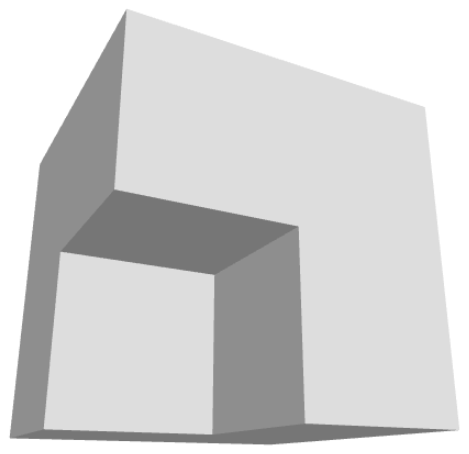
\includegraphics[width=5cm]{img/diffcube.png}
\end{center}
\vspace{-6mm}
\caption{Boolean difference of two cubes.}
\vspace{-1cm}
\label{fig:diffcube}
\end{figure}
\newpage

\subsection{Working with an interactive GUI vs. scripting}\label{subsec:scripting}

Virtually all production-level CAD systems such as SolidWorks, AutoCAD and 
others, come with a graphical user interface (GUI). There, the user 
can select objects from menus using the mouse, drag them on the computer 
screen, click into other menus to select their transformations, etc. 
These systems often automate some design tasks in order to make 
the professional designer as comfortable and as efficient as possible.
Each CAD system has some computational geometry engine, and the GUI can be 
viewed as a "remote control" to it. 

Another way to communicate with the computational geometry engine is via 
writing instructions in the form of short programs. These instructions 
do similar things that can be done via clicking in menus of a GUI. 
Such short programs are called {\em scripts}
and hence this technique is called {\em scripting}.

The philosophy of scripting is different from working with an interactive GUI. 
Let's assume for the moment that the user knows the Linux and Windows operating 
systems: Scripting is more like using Linux while working with an interactive 
GUI is more like using Windows. Linux users like to understand how things really work,
be in control, be able to change everything and anything if they want to. 
Of course this means less comfort and sometimes one has to deal with dirty details. 
People who like to just use things as they are, without knowing all the details, 
are better off with Windows. 

Another such analogy is between \LaTeX -- the most popular typesetting system for engineering 
and scientific literature -- and Microsoft Word. \LaTeX \,uses a scripting approach, Word is more
about clicking into menus. While both systems can be used to produce high quality documents, 
and many people love Word, many other people would say that they would never write a book in it. 

In the end the choice is up to the user. It is not our objective to advocate any
of these two approaches here. The fact that NCLab uses PLaSM has its roots in
the fact that it was created by people who love Linux and \LaTeX. Of course it would be possible 
to create an interactive GUI for PLaSM in NCLab as well, but this will be only done if there 
is enough demand.\\

\noindent
But back to scripting -- scripting puts more emphasis on the entire {\em design procedure}
than on the final design. In other words, the main difference between 
scripting and working with a GUI is not in the range of final designs that one can create 
-- it is in {\em how one creates them}. A script contains 
a complete sequence of steps, the history of the design process. It reveals clearly each 
operation as well as the order of operations. At any time, any step 
of the design process can be checked and adjusted. Scripts can be run and 
re-run as many times as needed, until the design (process) is perfect. 
Working with a scripting language such as PLaSM allows us to improve the entire  
{\em design workflow} and learn good habits, which might be desirable for
educational applications.

Clearly, the scripting approach is not as widely used (yet) as working with 
interactive graphical applications. Let us therefore mention a few 
additional aspects and benefits of scripting that may not be obvious 
to educators who use traditional CAD systems:


\begin{itemize}

\item Scripting is a more "bare" approach. It makes sure that students understand
      all geometrical operations, their parameters, and dependencies.
\item Parts of an existing design can be reused for other designs by copying the 
      corresponding lines of the script. 
\item Script can automate tedius tasks as well as allow parameters (variables)
      in the design. 
\end{itemize}
But let's stop talking and get to work! PLaSM makes it possible to define a wide range of 3D 
objects, transform them, subtract them from each other, create their intersections
and unions, define many different types of curved surfaces, solidify them, and 
much more. In no time, you will be able to create advanced 3D geometries such 
as the one shown in Fig. \ref{fig:vault0}.

\begin{figure}[!ht]
\begin{center}
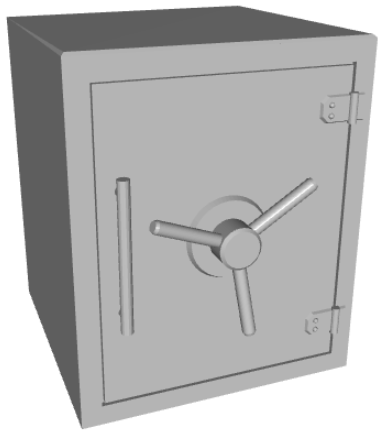
\includegraphics[width=0.4\textwidth]{img/vault.png}
\end{center}
\vspace{-4mm}
\caption{Vault model created with PLaSM.}
%\vspace{-1cm}
\label{fig:vault0}
\end{figure}


\subsection{Launching new PLaSM project}

The underlying cloud computing platform for this course is NCLab 
(http://nclab.com).
PLaSM scripts are sent to a remote server, evaluated there, 
and the results are sent back to your web browser. Your device uses
its graphics card for real-time rendering of 3D objects. For this 
reason, {\bf your web browser has to support WebGL}. 
New PLaSM project can be launched via the CAD icon on Desktop, as shown 
in Fig. \ref{fig:python}.
\newpage

\begin{figure}[!ht]
\begin{center}
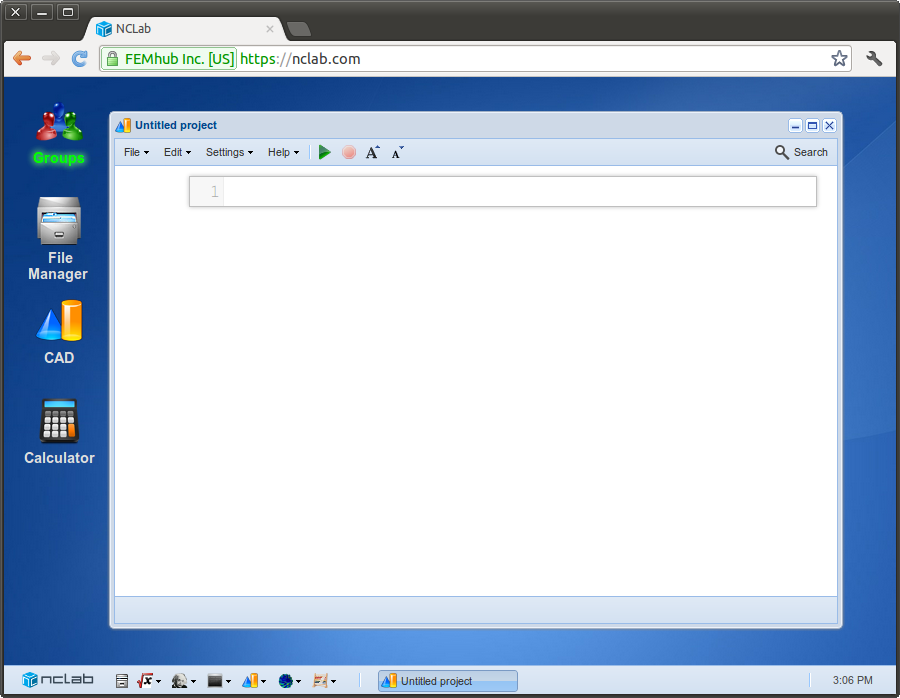
\includegraphics[width=0.5\textwidth]{img/python.png}
\end{center}
\vspace{-2mm}
\caption{Launching a new PLaSM project.}
\label{fig:python}
\end{figure}
\noindent
The WebGL technology is still experimental, so it may be disabled 
in your web browser by default. Even after you enable it, it may not work 
right out of the box. For this reason we provide a document called 
"WebGL and Its Problems" in the Help section.

\subsection{Hello, World!}

In the input cell, enter the code:
\begin{bluecode}
c = CUBE(1)
lab.view(c)
\end{bluecode}
\index{CUBE}
\index{lab.view}
\noindent
Here, {\tt CUBE} is a command that creates a cube of a given size and {\tt c} is the 
name of the newly created object. The name can be arbitrary as long as it does not conflict with 
any PLaSM command. To minimize name clashes, all PLaSM commands are CAPITALIZED.

After you are done typing the script, click on the green arrow button in the menu
or under the input cell. The former option will run all cells 
in the project, the latter only the particular cell. Pressing the green arrow sends 
the script to the server. If your Internet connection works, the answer  comes back 
instantly and a new WebGL widget displaying a unit cube in grey color will appear, as 
shown in Fig. \ref{fig:cube}. 
\newpage

\begin{figure}[!ht]
\begin{center}
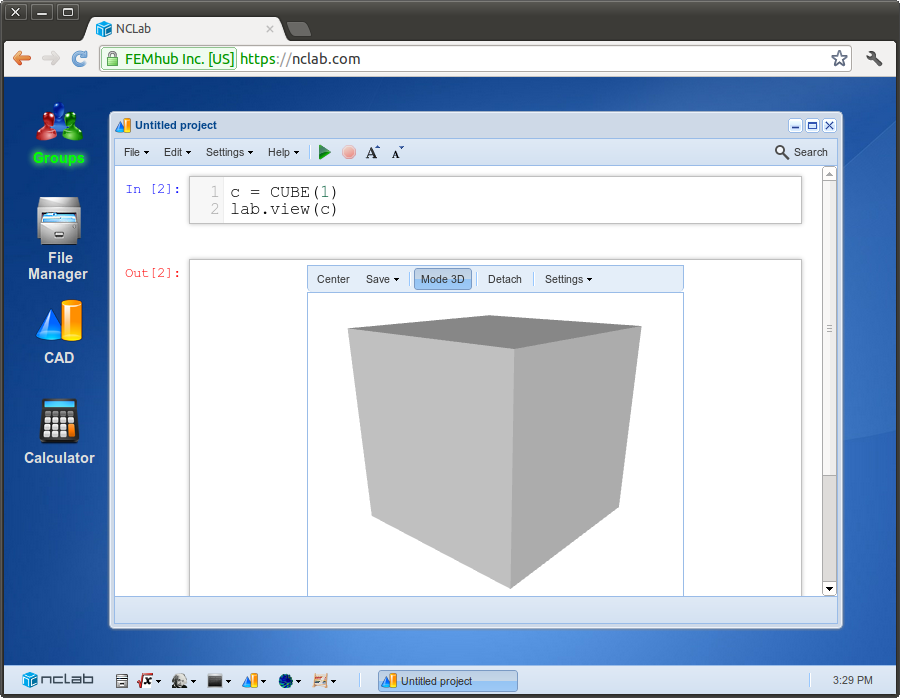
\includegraphics[width=0.5\textwidth]{img/cube.png}
\end{center}
\vspace{-2mm}
\caption{WebGL widget showing a unit cube that we created.}
\vspace{2mm}
\label{fig:cube}
\end{figure}
\noindent
Congratulations, you just created your first Solid Model!

\subsection{Mouse controls}

Now click into the window and move the mouse while holding the left
button down. The cube will rotate freely. Holding the middle
button (or the mouse wheel) pressed and moving the mouse will move the 
object in any direction. Zooming in and out is done via the mouse wheel 
or by holding the right-hand mouse button down and moving the mouse.
The latter option allows for finer zooming.

\subsection{RGB colors}

Before we move on to other 3D objects, adjust the code in the input cell to 
\begin{bluecode}
c = CUBE(1)
lab.view(c, [102, 230, 153])
\end{bluecode}
\index{CUBE}
\index{lab.view}
\noindent
The same could be done by creating a separate variable (called, say, {\tt col})
for the color and passing it into the {\tt lab.view()} function:

\begin{bluecode}
c = CUBE(1)
col = [102, 230, 153]
lab.view(c, col)
\end{bluecode}
Run the script again.
This will render the cube {\tt c} in a greenish color, as shown in 
Fig. \ref{fig:cube2}.
\newpage

\begin{figure}[!ht]
\begin{center}
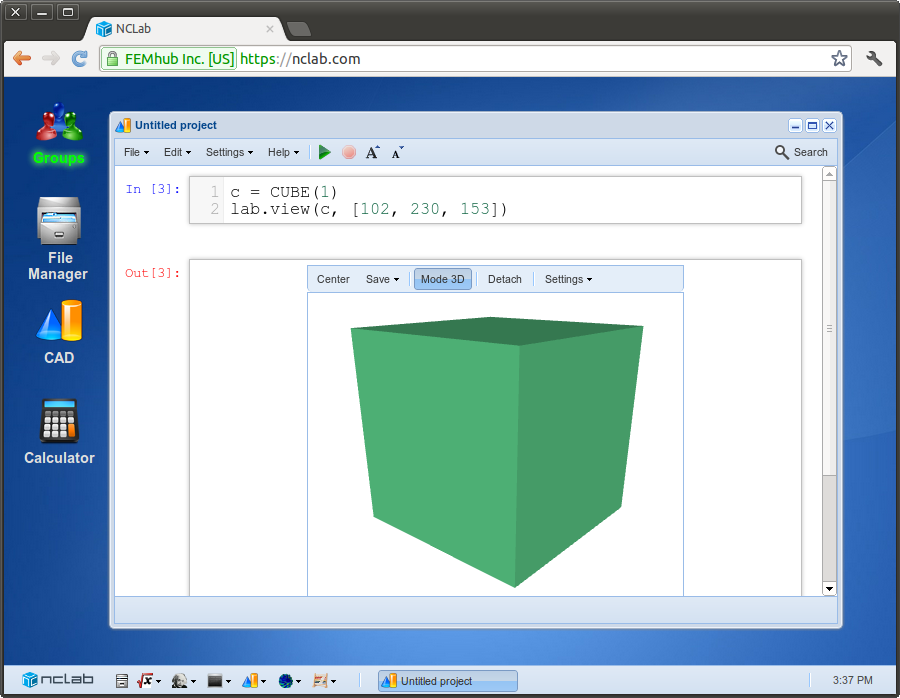
\includegraphics[width=0.5\textwidth]{img/cube2.png}
\end{center}
\vspace{-2mm}
\caption{Changing the cube's color.}
\vspace{2mm}
\label{fig:cube2}
\end{figure}
\noindent
The color can be further changed by redefining the triplet {\tt [102, 230, 153]}. 
If the triplet is omitted, the object is rendered using grey color. Each value can 
be an arbitrary integer between 0 and 255. Experiment for a while with various colors, keeping a few 
simple rules in mind:

\begin{itemize}
\item With just the first value being non-zero, such as in {\tt [150, 0, 0]},
      you get {\bf pure red}. The closer the value to 255, the lighter the color.
      This holds for all three components.
\item With just the second value being non-zero, such as in {\tt [0, 55, 0]},
      you obtain {\bf pure green}.
\item With just the third value being non-zero, such as in {\tt [0, 0, 222]},
      you will have {\bf pure blue}. 
\item Using three identical values will result into some shade of grey. For 
      example, {\tt [0, 0, 0]}
      means black and {\tt [255, 255, 255]} means white.
\item Varying all three numbers, you can get any color that you want. It is not 
      easy to translate a color, such as "purple", "cyan" or "orange" into the RGB
      values. But there are many web pages that will do it for you, such as for
      example http://kb.iu.edu/data/aetf.html. Just google for "rgb tables".
\end{itemize}
In Subsection \ref{subsec:multicolor} we will show how various objects in
one scene can be displayed using different colors.

\section{Creating Simple Objects}

\subsection{Objectives}
\begin{itemize}
\item Learn to create simple objects such as cubes, bricks, squares, rectangles, spheres, circles, 
      tetrahedra, triangles, prisms, cones, truncated cones, 
      cylinders, tubes, and toruses. 
\item Learn to always remember where objects are positioned in the coordinate system.
\item Understand the representation of curved surfaces.
\item Learn to create convex hulls.
\item Learn to extrude 2D objects to 3D.
\item Understand the benefits of scripting.
\end{itemize}
We will usually {\bf skip the command
{\tt lab.view()} in the following} since its presence is obvious.
The resulting object to be displayed will usually be called "out".

\subsection{Bricks, rectangles, and squares}

We already know that the command {\tt CUBE(a)} renders a 3D cube of
dimension {\tt a}. Analogously, command {\tt BRICK(a, b, c)} \index{BRICK}
renders a 3D brick of dimensions {\tt a}, {\tt b} and {\tt c}. 
Let us change the code in the input cell to  

\begin{bluecode}
out = BRICK(3.0, 2.0, 1.0)
\end{bluecode}
\index{BRICK}
and press the green arrow button. The result is displayed in Fig. \ref{fig:cuboid-1}.\\

\begin{figure}[!ht]
\begin{center}
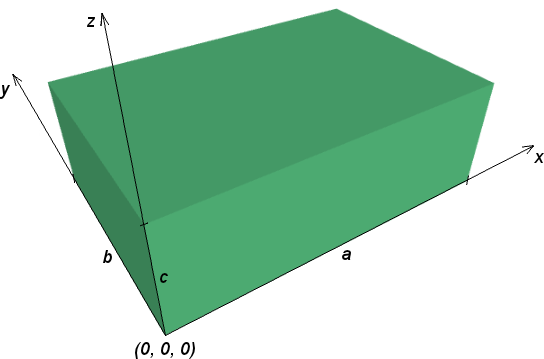
\includegraphics[width=0.62\textwidth]{img/cuboid-1.png}
\end{center}
\vspace{-4mm}
\caption{Brick of dimensions 3, 2 and 1.}
\label{fig:cuboid-1}
\end{figure}
\newpage

\noindent
{\bf Positioning of objects}.
Fig. \ref{fig:cuboid-1} also shows coordinate axes which are not
displayed in the WebGL widget. As you can see, the brick is positioned 
in the first quadrant, its edges are aligned with coordinate axes, and one 
vertex lies at the origin (0, 0, 0). To avoid mistakes when working with 
multiple objects, it is important to always remember where
each object is located in the global coordinate system. \\

\noindent
{\bf Rectangle} of dimensions {\tt a} and {\tt b} can be rendered typing 
{\tt RECTANGLE(a, b)}, as shown in Fig. \ref{fig:cuboid-2}.

\begin{figure}[!ht]
\begin{center}
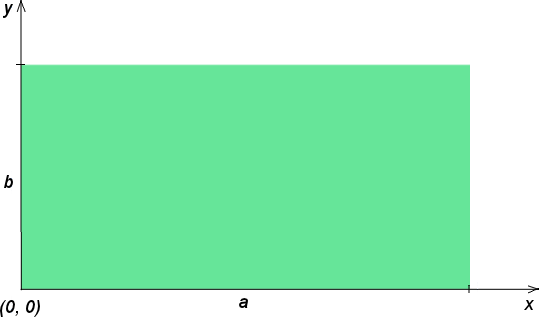
\includegraphics[width=0.6\textwidth]{img/cuboid-2.png}
\end{center}
\vspace{-4mm}
\caption{Rectangle of dimensions 2 and 1.}
\label{fig:cuboid-2}
%\vspace{-1cm}
\end{figure}
\noindent
Notice again that the rectangle is located in the first quadrant with its edges 
aligned with coordinate axes, and that its bottom-left vertex lies at the 
origin (0, 0). \\

\noindent
{\bf Square} of dimension {\tt a} can be constructed using the command {\tt SQUARE(a)}.  

\subsection{Tetrahedra and triangles}

The command {\tt TETRAHEDRON([a1, a2, a3], [b1, b2, b3], [c1, c2, c3], [d1, d2, d3])} renders 
a tetrahedron with the vertices {\tt [a1, a2, a3]}, {\tt [b1, b2, b3]}, {\tt [c1, c2, c3]}
and {\tt [d1, d2, d3]}. The output of the sample code

\begin{bluecode}
out = TETRAHEDRON([-2, 0, 0], [1, 0, 0], [0, 4, 1], [0, 1, 2])
\end{bluecode}
\index{TETRAHEDRON}
is shown in Fig. \ref{fig:chull}.

\begin{figure}[!ht]
\begin{center}

\includegraphics[width=0.35\textwidth]{img/chull.png}
\end{center}
\vspace{-4mm}
\caption{Tetrahedron with vertices [-2, 0, 0], [1, 0, 0], [0, 4, 1] and [0, 1, 2].}
\label{fig:chull}
%\vspace{-1cm}
\end{figure}
\newpage
\noindent
Analogously, the command {\tt TRIANGLE([a1, a2], [b1, b2], [c1, c2])} renders 
a triangle with the vertices {\tt [a1, a2]}, {\tt [b1, b2]} and {\tt [c1, c2]}. 

\subsection{Prisms}\label{subsec:prism}

Given a triangle {\tt B} and a positive number {\tt H}, the command 
{\tt PRISM(B, H)} renders a prism with the base {\tt B} and height {\tt H}. 
The output of the sample code

\begin{bluecode}
B = TRIANGLE([-1, 0], [1, 0], [0, -2])
H = 2.0
out = PRISM(B, H)
\end{bluecode}
\index{TRIANGLE}
\index{PRISM}
is shown in Fig. \ref{fig:prism}. The base {\tt B} can be any 2D polygon,
as we will see in Subsection \ref{subsec:extrusion}.\\

\begin{figure}[!ht]
\begin{center}
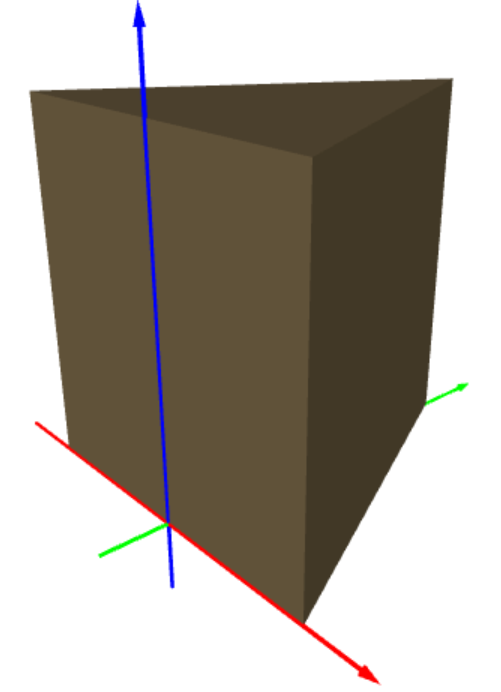
\includegraphics[width=0.27\textwidth]{img/prism-0.png}
\end{center}
\vspace{-4mm}
\caption{Prism with base {\tt B} and height {\tt H}.}
\label{fig:prism}
\vspace{-1cm}
\end{figure}
\newpage


\subsection{Spheres and circles}

Sphere of radius $R$ and center at (0, 0, 0) can be rendered using the command 
{\tt SPHERE(R)}. The output of the sample code

\begin{bluecode}
out = SPHERE(3.0)
\end{bluecode}
\index{SPHERE}
is shown in Fig. \ref{fig:sphere-1}.

\begin{figure}[!ht]
\begin{center}
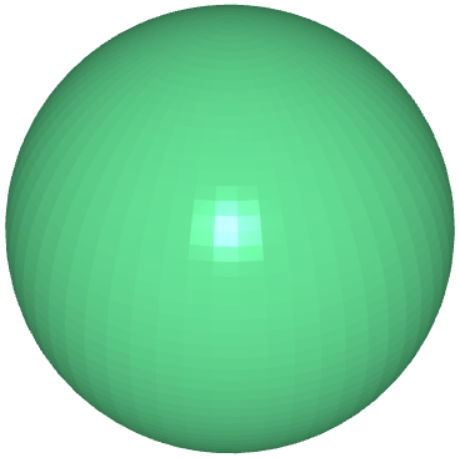
\includegraphics[width=0.35\textwidth]{img/sphere-1.png}
\end{center}
\vspace{-4mm}
\caption{Sphere of radius $R$ and center at (0, 0, 0).}
\label{fig:sphere-1}
%\vspace{-1cm}
\end{figure}
\noindent
Circle with radius $R$ and center at (0, 0), lying in the $xy$-plane 
can be defined using the command {\tt CIRCLE(R)}:

\begin{bluecode}
R = 5.0
out = CIRCLE(R)
\end{bluecode}
\index{CIRCLE}

\subsection{Approximation of curved surfaces} 

In PLaSM, curved surfaces such as the spherical one shown in Fig. \ref{fig:sphere-1}
are always approximated using linear segments. Each curved object comes
with a default division that the user can adjust if needed. For the 
{\tt SPHERE} command, the default divisions are 32 in the angular direction 
and 32 in the $z$-direction. The division can be used as an optional argument.
If there are two divisions, they are always enclosed in square brackets. Hence, 
the command

\begin{bluecode}
s = SPHERE(3.0)
\end{bluecode}
\index{SPHERE}
is equivalent to 

\begin{bluecode}
s = SPHERE(3.0, [32, 32])
\end{bluecode}
\index{SPHERE}
The default sphere is approximated using $32^2 = 1024$ linear
segments. If you decide to make it look better by using 
twice finer division in both directions,

\begin{bluecode}
s = SPHERE(3.0, [64, 64])
\end{bluecode}
\index{SPHERE}
then the number of linear segments jumps to $64^2 = 4096$. Making 
both divisions twice finer once more would yield $128^2 = 16384$ linear
segments. 

If you decide to make the surface representation finer, then you may experience 
slower rendering in your web browser as there simply is more data 
to transfer from the server. Once the object is in your web browser,
then real-time rendering (rotating, scaling, moving) is done by your 
graphic card, and thus it depends entirely on its power how smooth
it will be. One last aspect to consider is that for Boolean operations 
such as intersection of objects, that will be discussed later, the 
computational algorithm works with all linear segments of all objects. 
In this case, fine representation of curved surfaces put more workload 
on the server, which results in higher memory consumption and longer 
computing times. 

What we said above applies to circles as well. By default, every circle 
is approximated using an equilateral polygon 
with 64 edges. To change the number of edges for example to 32, type

\begin{bluecode}
c = CIRCLE(R, 32)
\end{bluecode}
\index{CIRCLE}

\subsection{Cylinders}

A cylinder of radius $R$ and height $H$ can be defined using 
the command {\tt CYLINDER(R, H)}. The cylinder's axis is in 
the $z$-direction, and the midpoint of its base circle is the 
origin (0, 0, 0). The output of the sample code

\begin{bluecode}
R = 0.25
H = 1.0
out = CYLINDER(R, H)
\end{bluecode}
\index{CYLINDER}
is shown in Fig. \ref{fig:cyl-1}.

\begin{figure}[!ht]
\begin{center}
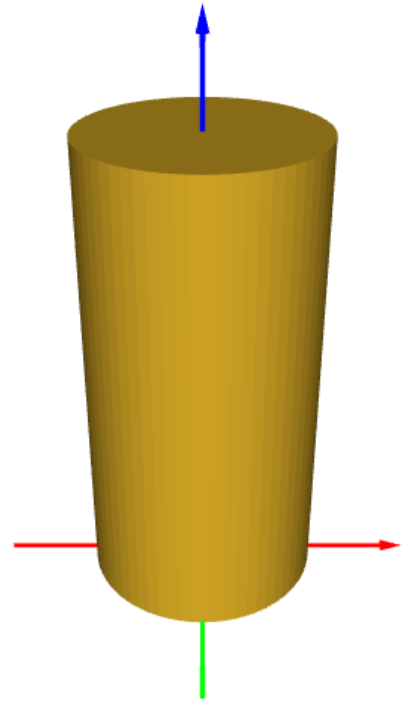
\includegraphics[width=0.3\textwidth]{img/cyl-1.png}
\end{center}
\vspace{-4mm}
\caption{Cylinder of radius $R$ and height $H$.}
\label{fig:cyl-1}
%\vspace{-1cm}
\end{figure}
\noindent
By default, the curved surface is split into 64 vertical linear segments. To 
change the division to another number {\tt M}, use

\begin{bluecode}
c = CYLINDER(R, H, M)
\end{bluecode}
\index{CYLINDER}

\subsection{Tubes}

Tube of inner radius $r$, outer radius $R$ and height
$H$ is rendered using the command {\tt TUBE(r, R, H)}. 
The tube is positioned in the global coordinate system 
as the cylinder -- its axis coincides with the $z$-axis and 
the center of its base is at (0, 0, 0). 
The output of the sample code

\begin{bluecode}
r = 0.9
R = 1.0
H = 3.0
out = TUBE(r, R, H)
\end{bluecode}
\index{TUBE}
is shown in Fig. \ref{fig:tube-1}.

\begin{figure}[!ht]
\begin{center}
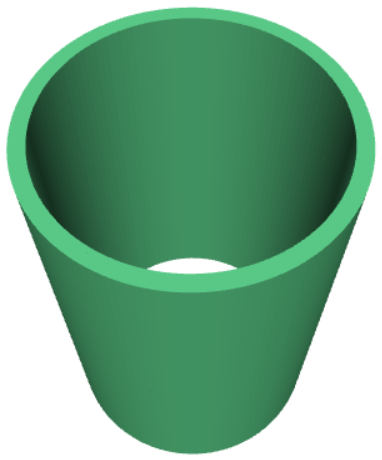
\includegraphics[width=0.3\textwidth]{img/tube-1.png}
\end{center}
\vspace{-4mm}
\caption{Tube of inner radius $r$, outer radius $R$ and height $H$.}
\label{fig:tube-1}
%\vspace{-1cm}
\end{figure}
\noindent
By default, the inner and outer curved surfaces are split each into 64 vertical 
linear segments. To change the division to another number {\tt M}, use

\begin{bluecode}
t = TUBE(r, R, H, M)
\end{bluecode}
\index{TUBE}

\subsection{Cones}\label{par:coco}

Cone of radius $R$ and height $H$ is defined using the command 
{\tt CONE(R, H)}. The cone's axis coincides with the $z$-axis and 
the center of the base circle lies at the origin (0, 0, 0).
The output of the sample code

\begin{bluecode}
R = 5
H = 10
out = CONE(R, H)
\end{bluecode}
\index{CONE}
\noindent
is shown in Fig. \ref{fig:convexhull-2a}.
\newpage

\begin{figure}[!ht]
\begin{center}
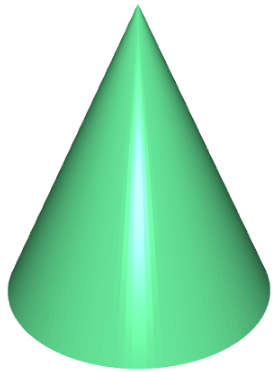
\includegraphics[width=0.27\textwidth]{img/convexhull-2.png}
\end{center}
\vspace{-4mm}
\caption{Cone of radius $R$ and height $H$.}
\label{fig:convexhull-2a}
%\vspace{-1cm}
\end{figure}
\noindent
By default, the curved surface is split into 64 triangular linear segments. To 
change the division to another number {\tt M}, use

\begin{bluecode}
c = CONE(R, H, M)
\end{bluecode}
\index{CONE}
By the way, the linear surface representation can be used 
to render various other objects. For example, the code 

\begin{bluecode}
out = CONE(R, H, 4)
\end{bluecode}
\index{CONE}
will render a pyramid shown in Fig. \ref{fig:cone-4}.

\begin{figure}[!ht]
\begin{center}
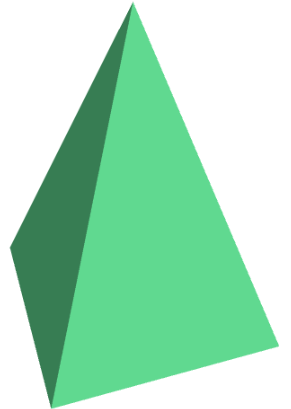
\includegraphics[width=0.27\textwidth]{img/cone-4.png}
\end{center}
\vspace{-4mm}
\caption{Pyramid rendered using the {\tt CONE} command.}
\label{fig:cone-4}
%\vspace{-1cm}
\end{figure}
\noindent
The same trick, of course, can be used with SPHERE, CYLINDER, TUBE and any 
other object that has curved boundary.
\newpage

\subsection{Truncated cones}

Truncated cone of base radius $R_1$, top radius $R_2$ and height $H$
can be constructed as follows:

\begin{bluecode}
R1 = 5.0
R2 = 2.5
H = 5.0
out = TRUNCONE(R1, R2, H)
\end{bluecode}
\index{TRUNCONE}
Screenshot of the result is shown in Fig. \ref{fig:tcone}.

\begin{figure}[!ht]
\begin{center}
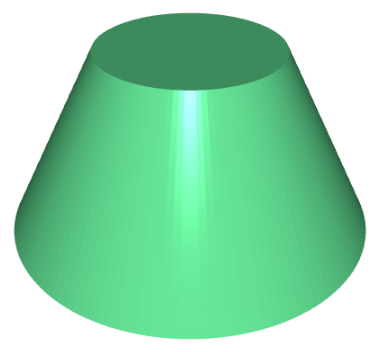
\includegraphics[width=0.35\textwidth]{img/tcone-8.png}
\end{center}
\vspace{-6mm}
\caption{Truncated cone.}
\label{fig:tcone}
%\vspace{-1cm}
\end{figure}
\noindent
By default, the curved surface is split into 64 trapezoidal linear segments. 
To change the division to another number {\tt M}, use

\begin{bluecode}
c = TRUNCONE(R1, R2, H, M)
\end{bluecode}
\index{TRUNCONE}
As a simple trick, we can construct a truncated pyramid:

\begin{bluecode}
out = TRUNCONE(R1, R2, H, 4)
\end{bluecode}
\index{TRUNCONE}
The output is shown in Fig. \ref{fig:tcone-9}.

\begin{figure}[!ht]
\begin{center}

\includegraphics[width=0.35\textwidth]{img/tcone-9.png}
\end{center}
\vspace{-6mm}
\caption{Truncated pyramid.}
\label{fig:tcone-9}
\vspace{-1cm}
\end{figure}
\newpage


\subsection{Toruses}

Command {\tt TORUS(r, R)} renders a torus with inner radius $r$ and outer 
radius $R$. It is used as follows:
\begin{bluecode}
r = 3.0
R = 5.0
out = TORUS(r, R)
\end{bluecode}
\index{TORUS}
The center of the torus is at the origin (0, 0, 0) and its axis
is the $z$-axis. This is illustrated in Fig. \ref{fig:torus-1}.

\begin{figure}[!ht]
\begin{center}
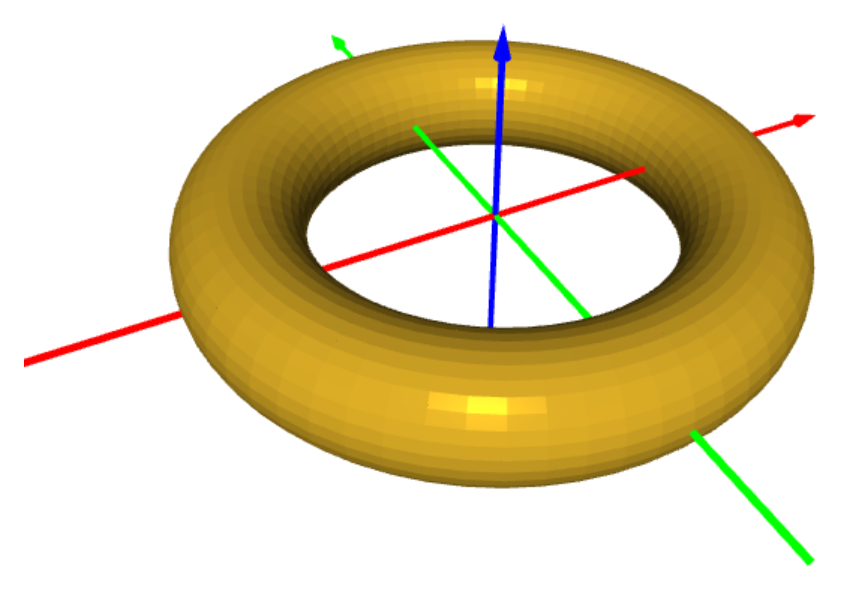
\includegraphics[width=0.6\textwidth]{img/torus-1.png}
\end{center}
\vspace{-4mm}
\caption{Torus with inner radius $r$, outer radius $R$ and center at the origin (0, 0, 0).}
\label{fig:torus-1}
%\vspace{-1cm}
\end{figure}
\noindent
By default, the major (large) circle is split into 64 linear segments and
the minor (small) one into 32. Thus the default command {\tt TORUS(r, R)} is
equivalent to {\tt TORUS(r, R, [64, 32])}. To change the divisions to other 
numbers {\tt [M, N]}, use

\begin{bluecode}
c = TORUS(R, H, [M, N])
\end{bluecode}
\index{TORUS}
Also here, the piecewise-linear surface representation can be used to
create objects that would be much more difficult to construct by other means.  
Fig. \ref{fig:torus-4} shows the output of the command {TORUS(3, 5, [64, 4])}.
\newpage

\begin{figure}[!ht]
\begin{center}
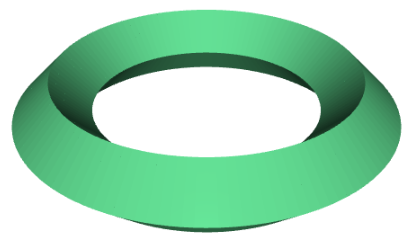
\includegraphics[width=0.5\textwidth]{img/torus-4.png}
\end{center}
\vspace{-4mm}
\caption{Output of the command {\tt TORUS(3, 5, [64, 4])}.}
\label{fig:torus-4}
%\vspace{-1cm}
\end{figure}
\noindent
Fig. \ref{fig:torus-5} shows the output of the command {TORUS(3, 5, [4, 64])}.\\

\begin{figure}[!ht]
\begin{center}
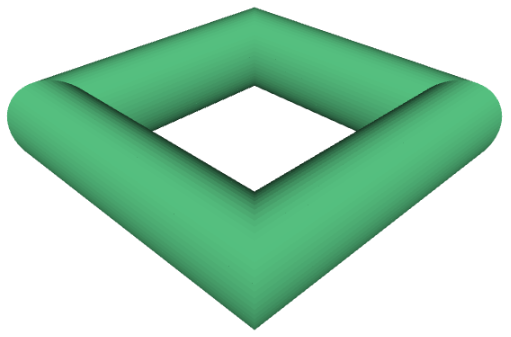
\includegraphics[width=0.5\textwidth]{img/torus-5.png}
\end{center}
\vspace{-4mm}
\caption{Output of the command {\tt TORUS(3, 5, [4, 64])}.}
\label{fig:torus-5}
%\vspace{-1cm}
\end{figure}
\noindent

\subsection{Convex hull}

Constructing convex hulls of finite point sets in 2D and 3D is one of the 
most important algorithms of computational geometry. A 2D or 3D object is {\em convex} if for any 
two points located inside, the straight line connecting the points 
lies entirely inside. For illustration, Fig. \ref{fig:convex} 
shows a convex object on the left and a non-convex one on the right.
\newpage

\begin{figure}[!ht]
\begin{center}
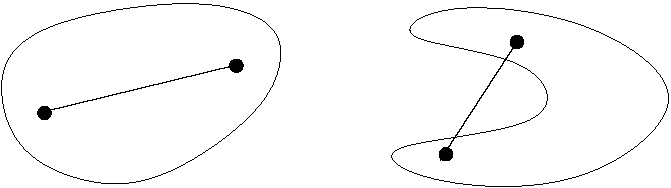
\includegraphics[width=0.82\textwidth]{img/convex.pdf}
\end{center}
\vspace{-4mm}
\caption{Convex 2D object (left) and a non-convex one (right), along with 
         sample straight lines connecting interior points.}
\label{fig:convex}
%\vspace{-1cm}
\end{figure}
\noindent
By {\em convex hull} of a set of 2D or 3D points we mean the smallest convext 
set that contains all the points. To construct convex hull of a large number 
of points efficiently is not a trivial task at all. It can be proven 
mathematically that the complexity of finding a convex hull of $n$ points 
is always at least $Ω(n \log n)$ where $n$ is the number of points 
 
The complexity of more recent convex hull algorithms can be characterized 
in terms of both input size $n$ and the output size $h$ (the number of vertices
of the hull). Such algorithms are called {\em output-sensitive algorithms}. 
They are often asymptotically more efficient than $Θ(n \log n)$ algorithms 
in cases when $h$ is much lower than $n$. 

The earliest output-sensitive 
algorithm was introduced by Kirkpatrick and Seidel in 1986 (who 
called it "the ultimate convex hull algorithm"). A much simpler algorithm 
was developed by Chan in 1996, and is called Chan's algorithm. The latter
is used in PLaSM. \\

\noindent
The {\tt CONVEXHULL} command (that can be abbreviated as {\tt CHULL} or {\tt CH})
takes a set of points and creates their convex hull:

\begin{bluecode}
out = CONVEXHULL([-1, 0], [1, 0], [0.5, 1], [-0.5, 1])
\end{bluecode}
\index{CONVEXHULL}
This code renders a 2D trapezoid spanning the points (-1, 0), (1, 0), (0.5, 1) and 
(-0.5, 1). The code

\begin{bluecode}
out = CONVEXHULL([-1, -1, 0], [1, -1, 0], [1, 1, 0], [-1, 1, 0], [0, 0, 1])
\end{bluecode}
\index{CONVEXHULL}
creates a 3D pyramid with base square (-1, 1)$\times$(-1, 1) and height 1,
as shown in Fig. \ref{fig:pyra}. 

\begin{figure}[!ht]
\begin{center}

\includegraphics[width=0.3\textwidth]{img/pyra.png}
\end{center}
\vspace{-4mm}
\caption{3D pyramid constructed as a convex hull.}
\label{fig:pyra}
\vspace{-1cm}
\end{figure}
\newpage
\noindent
If the user already has a list of points, defined for example as

\begin{bluecode}
L = [[-1, -1, 0], [1, -1, 0], [1, 1, 0], [-1, 1, 0], [0, 0, 1]]
\end{bluecode}
then the way to use the {\tt CONVEXHULL} command is by inserting 
an asterisk '*' in front of the name of the list: 

\begin{bluecode}
out = CONVEXHULL(*L)
\end{bluecode}
\index{CONVEXHULL}


\subsection{Dodecahedron}

A unit dodecahedron is created as follows:

\begin{bluecode}
out = DODECAHEDRON
\end{bluecode}
\index{DODECAHEDRON}
The output is shown in Fig. \ref{fig:dodeca}.

\begin{figure}[!ht]
\begin{center}
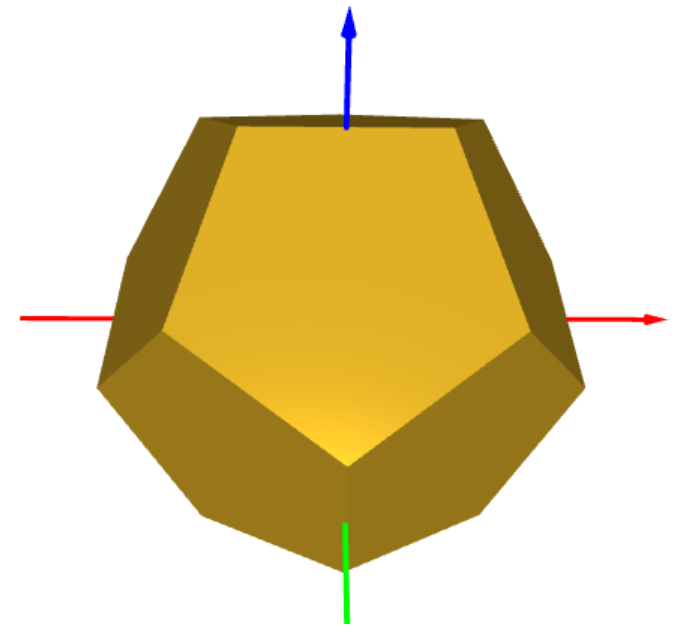
\includegraphics[width=0.35\textwidth]{img/dodeca-2.png}
\end{center}
\vspace{-4mm}
\caption{Dodecahedron.}
\label{fig:dodeca}
%\vspace{-1cm}
\end{figure}

\subsection{Icosahedron}

A unit icosahedron created via

\begin{bluecode}
out = ICOSAHEDRON
\end{bluecode}
\index{ICOSAHEDRON}
is shown in Fig. \ref{fig:icosa}.
\newpage
\begin{figure}[!ht]
\begin{center}
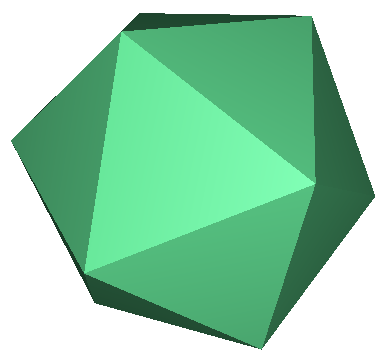
\includegraphics[width=0.35\textwidth]{img/icosa-2.png}
\end{center}
\vspace{-4mm}
\caption{Icosahedron.}
\label{fig:icosa}
%\vspace{-1cm}
\end{figure}

\subsection{Extrusion of 2D objects to 3D}\label{subsec:extrusion}

2D objects that lie in the $xy$-plane can be extruded to 3D
using the {\tt PRISM} command that we know from Subsection \ref{subsec:prism}. 
As an example, let us extrude a 2D polygon obtained as a convex hull.

\begin{bluecode}
B = CONVEXHULL([0, 0], [2, 0], [1, 2], [-1, 2])
H = 0.5
out = PRISM(B, H)
\end{bluecode}
\index{CONVEXHULL}
\index{PRISM}
The output is shown in Fig. \ref{fig:extrusion-3}.\\

\begin{figure}[!ht]
\begin{center}
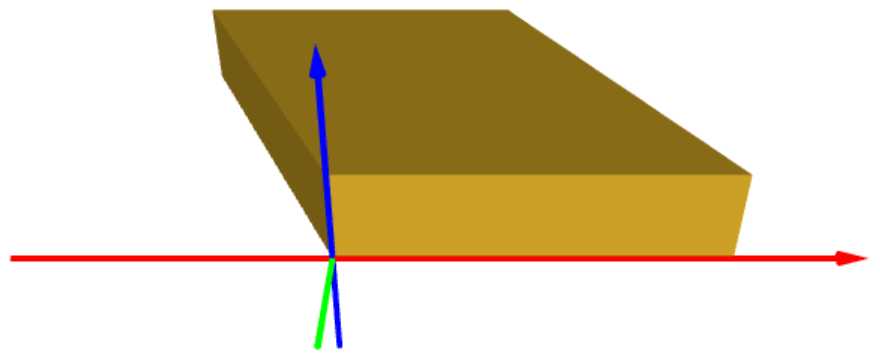
\includegraphics[width=0.4\textwidth]{img/extrude-3.png}
\end{center}
\vspace{-4mm}
\caption{Extrusion of a quadrilateral to 3D.}
\label{fig:extrusion-3}
%\vspace{-1cm}
\end{figure}
\noindent
The command {\tt PRISM(B, H)} uses a single interval in the $z$-direction. For future
reference, let us also introduce the command {\tt EXTRUDE(N, B, H)} that yields the same
extruded geometry as the {\tt PRISM} command, but subdivides the extrusion height {\tt H}
into {\tt N} equally long subintervals. 

\subsection{Grids and Cartesian products}\label{subsec:grids}

PLaSM provides useful commands {\tt GRID} and {\tt POWER} that 
make it easy to work with grids and Cartesian product geometries. The command
{\tt GRID} takes a list of positive and negative numbers where the 
positive ones stand for intervals (more precisely for their lengths) 
and negative for the lengths of spaces between the intervals. The 
intervals and spaces are placed on the right of the origin in the 
real axis. For example, 

\begin{bluecode}
GRID([2])
\end{bluecode}
\index{GRID}
renders a single interval (0, 2). The command

\begin{bluecode}
GRID([1, -3, 2])
\end{bluecode}
\index{GRID}
renders two intervals (0, 1) and (4, 6), leaving an empty 
space of length 3 between them. There is no limit of the 
length of the list.
The command  

\begin{bluecode}
grid_2d = POWER(grid1, grid2)
\end{bluecode}
\index{POWER}
creates a 2D object in the $xy$-plane that is the Cartesian 
product of the two grids. This 2D object can be multiplied 
with a third grid in the $z$-direction:

\begin{bluecode}
grid_3d = POWER(grid_2d, grid2)
\end{bluecode}
\index{POWER}
The result is a 3D solid object that is the Cartesian product 
of the three one-dimensional grids. This object can be scaled, 
translated, and rotated as any other solid object (to be discussed
in the next Section).

For illustration, consider the following script:

\begin{bluecode}
g1 = GRID([3, -1, 3, -1, 3, -1, 3])
g2 = GRID([2, -1, 2, -1, 2])
g3 = GRID([1, -1, 1])

planar_grid = POWER(g1, g2)
out = POWER(planar_grid, g3)
\end{bluecode}
\index{GRID}
\index{POWER}
The resulting Cartesian product solid is shown in Fig. \ref{fig:grid1}.\\

\begin{figure}[!ht]
\begin{center}
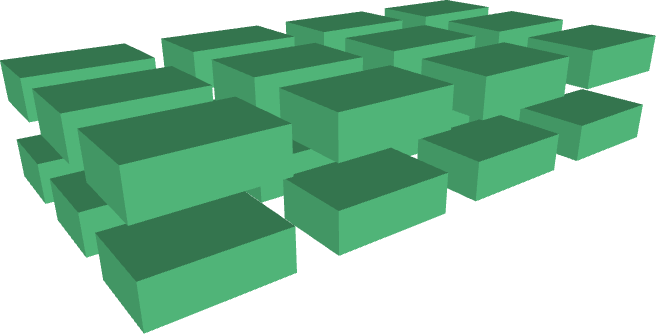
\includegraphics[width=0.6\textwidth]{img/grid1.png}
\end{center}
\vspace{-4mm}
\caption{Cartesian product geometry.}
\label{fig:grid1}
\vspace{-1cm}
\end{figure}
\newpage
\noindent
 


%%%%%%%%%%%%%%%%%%%%%%%%%%%%%%%%%%%%%%%%%%%%%%%%%%%%%%%%%%%%%%%%%%%%%%%%%%%%%%%
\section{Basic Transformations}

\subsection{Objectives}
\begin{itemize}
\item Learn to scale, translate, and rotate objects.
\item Learn to display multiple objects at once.
\item Learn to move objects above and below each other.
\item Learn to perform more general alignment operations.
\end{itemize}
So far we have learned how to create a variety of simple 2D and 3D objects. 
The next step is to learn how to transform them in a variety of ways. PLaSM
provides simple commands for that. 

\subsection{Scaling}

The command {\tt SCALE(obj, sx, sy, sz)} that can be abbreviated as 
{\tt S(obj, sx, sy, sz)} has four arguments: a 2D or 3D geometrical object {\tt obj} 
and scaling factors in the $x$, $y$ and $z$ directions. The scaling is done by
multiplying the $x$-coordinate of each point in the object by {\tt sx}, $y$-coordinates
by {\tt sy}, and $z$-coordinates by {\tt sz}. Default value 1.0 is used for directions where 
the object is not scaled. It is important to keep in mind that unless 
one side of the scaled object is aligned with zero in the direction of scaling, 
the object is not only scaled but it also moves. This is a consequence of the 
fact that the {\tt SCALE} command multiplies point coordinates, as we explained above. 
Let us also mention the command {\tt SIZE(obj, i)} that returns the length of 
the object {\tt obj} in the i-th spatial direction.
\index{SCALE}
\index{SIZE}
We can illustrate the {\tt SCALE} command on a cylinder {\tt cyl} of radius 1.0 
and height 0.3:

\begin{bluecode}
cyl = CYLINDER(1.0, 0.3)
\end{bluecode}
\index{CYLINDER}
As we know, the axis of this cylinder coincides with the $z$-axis 
and that the center of its bottom face is at (0, 0, 0). This cylinder is shown 
in Fig. \ref{fig:scale-0}.

\begin{figure}[!ht]
\begin{center}
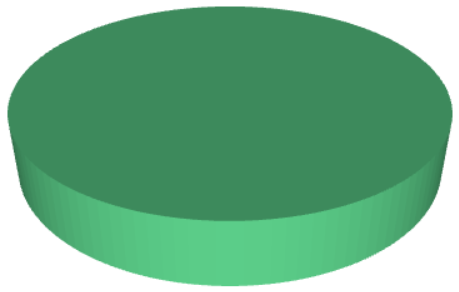
\includegraphics[width=0.35\textwidth]{img/scale-0.png}
\end{center}
\vspace{-4mm}
\caption{Cylinder of radius 1.0 and height 0.3.}
\label{fig:scale-0}
%\vspace{-1cm}
\end{figure}

\noindent
\underline{\em Scaling in $x$-direction}\\

First let us scale the cylinder in the $x$-direction by the factor of 2.0: 

\begin{bluecode}
out = SCALE(cyl, 2.0, 1.0, 1.0)
\end{bluecode}
\index{SCALE}
\newpage
The output is shown in Fig. \ref{fig:scale-1}.

\begin{figure}[!ht]
\begin{center}
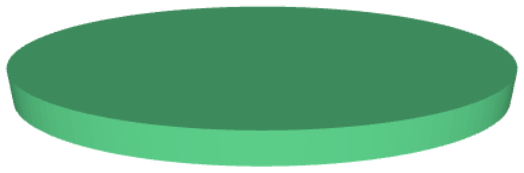
\includegraphics[width=0.6\textwidth]{img/scale-1.png}
\end{center}
\vspace{-4mm}
\caption{Cylinder {\tt cyl} scaled in the $x$-direction by 2.0.}
\label{fig:scale-1}
%\vspace{-1cm}
\end{figure}

\noindent
\underline{\em Scaling in $y$-direction}\\

The following command will 
scale the cylinder in the $y$-direction by the factor of 2.0: 

\begin{bluecode}
out = SCALE(cyl, 1.0, 2.0, 1.0)
\end{bluecode}
\index{SCALE}
The output is shown in Fig. \ref{fig:scale-2}.


\begin{figure}[!ht]
\begin{center}
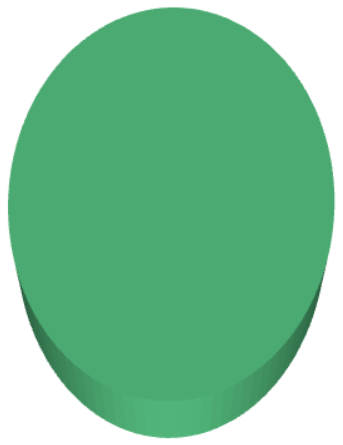
\includegraphics[width=0.35\textwidth]{img/scale-2.png}
\end{center}
\vspace{-4mm}
\caption{Cylinder {\tt cyl} scaled in the $y$-direction by 2.0.}
\label{fig:scale-2}
%\vspace{-1cm}
\end{figure}

\noindent
\underline{\em Scaling in $z$-direction}\\

The following command will 
scale the cylinder in the $z$-direction by the factor of 2.0: 

\begin{bluecode}
out = SCALE(cyl, 1.0, 1.0, 2.0)
\end{bluecode}
\index{SCALE}
The output is shown in Fig. \ref{fig:scale-3}.
\newpage

\begin{figure}[!ht]
\begin{center}
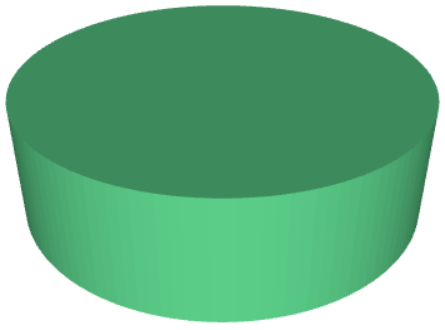
\includegraphics[width=0.35\textwidth]{img/scale-3.png}
\end{center}
\vspace{-4mm}
\caption{Cylinder {\tt cyl} scaled in the $z$-direction by 2.0.}
\label{fig:scale-3}
%\vspace{-1cm}
\end{figure}

\noindent
\underline{\em Scaling in multiple directions simultaneously}\\

Of course we can also scale the cylinder in two or three spatial directions 
simultaneously. For example, let us do it in the $x$-direction 
by 2.0 and in the $z$-direction by 4.0:

\begin{bluecode}
out = SCALE(cyl, 2.0, 1.0, 4.0)
\end{bluecode}
\index{SCALE}
The output is shown in Fig. \ref{fig:scale-4}.


\begin{figure}[!ht]
\begin{center}
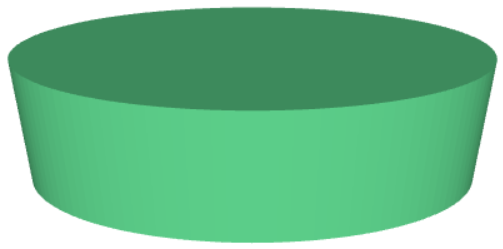
\includegraphics[width=0.5\textwidth]{img/scale-4.png}
\end{center}
\vspace{-4mm}
\caption{Cylinder {\tt cyl} scaled in the $x$ and $z$ directions by 2.0 and 4.0, respectively.}
\label{fig:scale-4}
%\vspace{-1cm}
\end{figure}

\subsection{Translations} \label{sec:translate}

The command {\tt TRANSLATE(obj, tx, ty, tz)} that can be abbreviated as 
{\tt T(obj, tx, ty, tz)} moves a 2D or 3D geometrical object {\tt obj} by {\tt tx}, {\tt ty},
{\tt tz} in the $x$, $y$ and $z$ directions, respectively. To practice
a little, let us create a unit cube and move it by 1.5 in the $x$-direction:

\begin{bluecode}
c = CUBE(1.0)
c2 = T(c, 1.5, 0.0, 0.0)
\end{bluecode}
\index{CUBE}
\index{TRANSLATE}
Next, let us create a sphere and move it simultaneously 
in the $x$-direction by 1.0 and in the $y$-direction by 2.0:

\begin{bluecode}
s = SPHERE(1.0)
s2 = T(s, 1.0, 2.0, 0.0)
\end{bluecode}
\index{SPHERE}
\index{TRANSLATE}
And last, we move the sphere {\tt s} simultaneously by -1.0 in the $x$-direction, 
by 1.0 in the $y$-direction and by 4.0 in the $z$-direction:

\begin{bluecode}
s = SPHERE(1.0)
s3 = T(s, -1.0, 1.0, 4.0)
\end{bluecode}
\index{SPHERE}
\index{TRANSLATE}

\subsection{Displaying multiple objects at once} \label{subsec:mo}

Often we need to view multiple objects at once, without 
the necessity to create their union as a new object. For 
this we can use the command {\tt STRUCT}. This command 
expects a list of geometrical objects. The following 
code creates three cubes and displays them all together:

\begin{bluecode}
c = CUBE(2.0)
c2 = T(c, 1.0, 1.0, 2.0)
c3 = T(c2, 1.0, 1.0, 2.0)
out = STRUCT(c, c2, c3)
\end{bluecode}
\index{CUBE}
\index{STRUCT}
\index{TRANSLATE}
The output is shown in Fig. \ref{fig:comp-1}

\begin{figure}[!ht]
\begin{center}

\includegraphics[width=0.35\textwidth]{img/comp-1.png}
\end{center}
\vspace{-4mm}
\caption{Multiple objects can be displayed at once using the STRUCT command.}
\label{fig:comp-1}
%\vspace{-1cm}
\end{figure}


\subsection{Moving objects above and below each other}

The command {\tt TOP(obj1, obj2)} is a higher-level command that 
moves object {\tt obj2} above object {\tt obj1}. 
For illustration, let us move a sphere above a cube:

\begin{bluecode}
c = CUBE(2.0)
s = SPHERE(1.0)
out = TOP(c, s)
\end{bluecode}
\index{CUBE}
\index{SPHERE}
\index{TOP}
The output is shown in Fig. \ref{fig:top-1}.

\begin{figure}[!ht]
\begin{center}
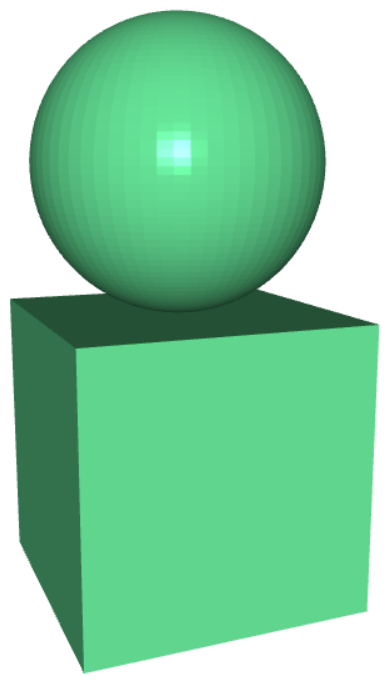
\includegraphics[width=0.2\textwidth]{img/top-1.png}
\end{center}
\vspace{-4mm}
\caption{Moving the sphere above the cube.}
\label{fig:top-1}
%\vspace{-1cm}
\end{figure}
\noindent
Fig. \ref{fig:bottom-1} shows the output of the script

\begin{bluecode}
c = CUBE(2.0)
s = SPHERE(1.0)
out = BOTTOM(c, s)
\end{bluecode}
\index{CUBE}
\index{SPHERE}
\index{BOTTOM}
that uses the {\tt BOTTOM} command to move the sphere 
under the cube.

\begin{figure}[!ht]
\begin{center}
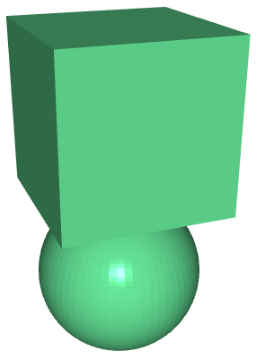
\includegraphics[width=0.23\textwidth]{img/bottom-1.png}
\end{center}
\vspace{-4mm}
\caption{Moving the sphere under the cube.}
\label{fig:bottom-1}
%\vspace{-1cm}
\end{figure}
\noindent

\subsection{More general alignment operations}

The {\tt TOP} and {\tt BOTTOM} commands that we met in the last subsection 
were special cases of the more general {\tt ALIGN} command. To understand it, 
let us rewrite the last two scripts without the {\tt TOP} and {\tt BOTTOM}
commands. The script 

\begin{bluecode}
c = CUBE(2.0)
s = SPHERE(1.0)
out = TOP(c, s)
\end{bluecode}
\index{CUBE}
\index{SPHERE}
\index{TOP}
can be written equivalently as

\begin{bluecode}
c = CUBE(2.0)
s = SPHERE(1.0)
out = ALIGN(c, s, [1, MID, MID], [2, MID, MID], [3, MAX, MIN])
\end{bluecode}
\index{CUBE}
\index{SPHERE}
\index{ALIGN}
This means that in the first axial direction ($x$-direction), the MIDpoint of {\tt c} is matched 
with the MIDpoint of {\tt s}. Same in the second axial direction ($y$-direction), In the 
third axial direction ($z$-direction), the MAXimum of {\tt c} is matched with the MINimum of {\tt s}.
This means that {\tt s} is centered on top of {\tt c}! Now it is easy to see that the 
script 

\begin{bluecode}
c = CUBE(2.0)
s = SPHERE(1.0)
out = BOTTOM(c, s)
\end{bluecode}
\index{CUBE}
\index{SPHERE}
\index{BOTTOM}
does the same as 

\begin{bluecode}
c = CUBE(2.0)
s = SPHERE(1.0)
out = ALIGN(c, s, [1, MID, MID], [2, MID, MID], [3, MIN, MAX])
\end{bluecode}
\index{CUBE}
\index{SPHERE}
\index{ALIGN}
While centering in the $x$ and $y$ directions has not changed, in the $z$-direction 
the MINimum of {\tt c} is matched with the MAXimum of {\tt s}. In other words,
{\tt s} is centered right below {\tt c}. 

Importantly -- only the second argument of the {\tt ALIGN} command, in our case the sphere {\tt s}, moves. The first 
object in the {\tt ALIGN} command stays exactly where it was. Furthermore, not all spatial directions 
have to be used in the {\tt ALIGN} command. If the triplet corresponding to some spatial direction 
is not used, the object is not moved in that direction. 

Let us complete this subsection by mentioning that PLaSM has a couple of additional
predefined alignment commands. The command {\tt LEFT(c, s)} is equivalent to

\begin{bluecode}
LEFT(c, s) = ALIGN(c, s, [1, MIN, MAX], [3, MIN, MIN])
\end{bluecode}
\index{LEFT}
Command {\tt RIGHT(c, s)} is the same as

\begin{bluecode}
RIGHT(c, s) = ALIGN(c, s, [1, MAX, MIN], [3, MIN, MIN])
\end{bluecode}
\index{RIGHT}
There is also the command {\tt UP(c, s)} defined as

\begin{bluecode}
UP(c, s) = ALIGN(c, s, [2, MAX, MIN], [3, MIN, MIN])
\end{bluecode}
\index{UP}
And last, the command {\tt DOWN(c, s)} is equivalent to

\begin{bluecode}
DOWN(c, s) = ALIGN(c, s, [2, MIN, MAX], [3, MIN, MIN])
\end{bluecode}
\index{DOWN}

\subsection{Rotations}

Objects can be rotated using the command {\tt ROTATE(obj, axis, angle)} 
that can be abbreviated as {\tt R(obj, axis, angle)}. Here {\tt obj} is
the geometrical object to be rotated, {\tt axis} is a number between 
1 and 3 that means the axis of rotation, and {\tt angle} is the angle of 
rotation. For 2D objects in the $xy$-plane, use {\tt axis = 3}. The axis of rotation 
always passes through the origin (0, 0, 0), so it is important 
to know exactly where your object is located. 

For example, when a CUBE is created, its center does not lie
at the origin of the coordinate system (0, 0, 0) -- the cube will 
rotate about one of its edges. Look at the following script 

\begin{bluecode}
c = CUBE(1.0)
c2 = R(c, 3, PI)
out = STRUCT(c, c2)
\end{bluecode}
\index{CUBE}
\index{ROTATE}
\index{STRUCT}
whose output is shown in Fig. \ref{fig:rot-1}. Clearly the axis of 
rotation is where the two cubes meet. 

\begin{figure}[!ht]
\begin{center}
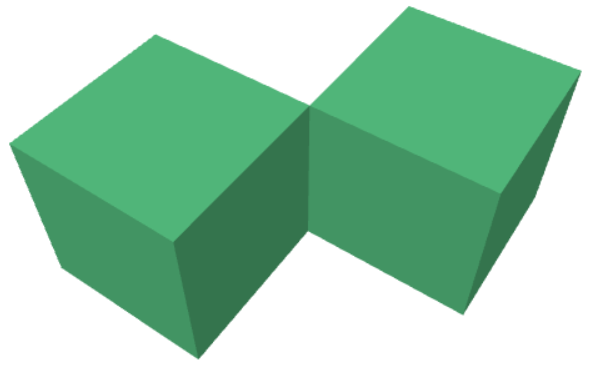
\includegraphics[width=0.5\textwidth]{img/rot-1.png}
\end{center}
\vspace{-4mm}
\caption{Unit cube rotated by $\pi$ (180 degrees) shown together with the original unit cube.}
\label{fig:rot-1}
%\vspace{-1cm}
\end{figure}
\noindent
If we wanted to 
rotate the cube "in place", so that its center would not be moved,
we would have to first translate the cube in such a way that its center
lies at the origin. Let's do this. After moving the cube so that 
its center is at (0, 0, 0), we will rotate it in two different directions,
then move it by 2.0 in the $x$-direction and display along with 
the original cube for comparison:

\begin{bluecode}
c = CUBE(1.0)
c2 = R(c, 3, PI/4)
c2 = R(c2, 1, PI/4)
c2 = T(c2, 1, 1, 1)
out = STRUCT(c, c2)
\end{bluecode}
\index{CUBE}
\index{ROTATE}
\index{TRANSLATE}
\index{STRUCT}
The output is shown in Fig. \ref{fig:rot-2}.
\newpage

\begin{figure}[!ht]
\begin{center}

\includegraphics[width=0.35\textwidth]{img/rot-2.png}
\end{center}
\vspace{-4mm}
\caption{Cube rotated in two directions, moved, and displayed along with the original cube.}
\label{fig:rot-2}
%\vspace{-1cm}
\end{figure}

\subsection{Using multiple colors in one scene} \label{subsec:multicolor}

When multiple objects are shown at the same time, it may be useful
to use different colors for them.
This is very simple. Let us return to the example with three cubes 
from Subsection \ref{subsec:mo}. This is the original script,
showing three green cubes:

\begin{bluecode}
c = CUBE(2.0)
c2 = T(c, 1.0, 1.0, 2.0)
c3 = T(c2, 1.0, 1.0, 2.0)
out = STRUCT(c, c2, c3)
lab.view(out)
\end{bluecode}
\index{CUBE}
\index{STRUCT}
\index{TRANSLATE}
Let us define three colors {\tt red = [200, 0, 0]}, {\tt green = [0, 200, 0]}
and {\tt blue = [0, 0, 200]}, and color each cube with one of them:

\begin{bluecode}
c = CUBE(2.0)
red = [200, 0, 0]
c2 = T(c, 1.0, 1.0, 2.0)
green = [0, 200, 0]
c3 = T(c2, 1.0, 1.0, 2.0)
blue = [0, 0, 200]
lab.view([c, red], [c2, green], [c3, blue])
\end{bluecode}
\index{CUBE}
\index{STRUCT}
\index{TRANSLATE}
\noindent
In other words, the {\tt lab.view()} function can accept pairs {\tt [object, color]} separated
by commas. The output of the last script is shown in Fig. \ref{fig:comp-1k}.

\begin{figure}[!ht]
\begin{center}
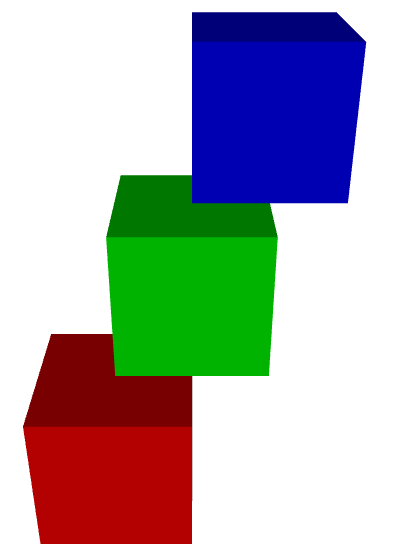
\includegraphics[width=0.39\textwidth]{img/multicolor-1.png}
\end{center}
\vspace{-4mm}
\caption{Using multiple colors.}
\label{fig:comp-1k}
%\vspace{-1cm}
\end{figure}



\section{Boolean Operations}

\subsection{Objectives}
\begin{itemize}
\item Understand the relation between geometry and logic.
\item Learn to subtract objects from each other.
\item Create union and intersection of objects.
\item Create exclusive or (xor) of objects.
\item Understand how to perform Boolean operations efficiently.
\end{itemize}

\subsection{Logic, sets, and geometry}

Finding logical operations in geometry may seem surprizing at first, but there 
is a simple explanation. Logical operations are used to 
work with {\em sets} in {\em set theory}, and 2D and 3D objects are nothing 
but sets of points. But first let us take a look at two simpler sets: 
Set $A$ of all integers between $1$ and $20$ that are divisible by two,

$$
A = \{2, 4, 6, 8, 10, 12, 14, 16, 18, 20\},
$$
and set $B$ of all integers between $1$ and $20$ that are divisible by three,

$$
B = \{3, 6, 9, 12, 15, 18\}.
$$
\underline{\em Set difference}

How do we define $A$ minus $B$? By taking all numbers from $A$ 
and removing those that are also present in $B$. Those are shown in red: 

$$
A = \{2, 4, {\color{red}6,} \,8, 10, {\color{red}12,} \,14, 16, {\color{red}18,} \,20\}.
$$
After removing them, we obtain a new set

$$
C = A \setminus B = \{2, 4, 8, 10, 14, 16, 20\}
$$
(the symbol '$\setminus$' is the standard way to write "minus" for sets).
Now where is the logic? The set $C$ is formed by \\

\centerline{
"all numbers that belong to $A$ {\color{red}and} at the same time they do {\color{red}not} belong to $B$".
}
\vspace{4mm}
\noindent
The words {\color{red}and}, {\color{red}not} stand for logical operations. 
The above statement can be written in a more compact form \\

\centerline{
"$C = A$ {\color{red}and} {\color{red}not}$(B)$".
}
\vspace{4mm}
\noindent
How does this apply to 2D and 3D geometrical objects? As we said above,
they are nothing but sets of points. If $A$ and $B$ are two geometrical objects,
then $A \setminus B$ is defined as\\

\centerline{
"all points that belong to $A$ {\color{red}and} at the same time they do {\color{red}not} belong to $B$".
}
\vspace{4mm}
\noindent
In Subsection \ref{subsec:subtract} we will explain in detail how this is done 
in PLaSM, and show examples. Now let us look at other set operations.\\

\noindent
\underline{\em Set union}

Staying with the sets $A$ and $B$ from above, their union is defined 
as the set of \\

\centerline{
"all numbers that belong to $A$ {\color{red}or} to $B$".
}
\vspace{4mm}
\noindent
In short,\\

\centerline{
"$C = A$ {\color{red}or} $B$".
}
\vspace{4mm}
\noindent
Here is how the set $C$ looks like:

$$
C = A \cup B = \{2, 3, 4, 6, 8, 9, 10, 12, 14, 15, 16, 18, 20\}
$$
(the symbol '$\cup$' is the standard way to denote set union). If $A$
and $B$ are geometrical objects, then their union is the set of \\

\centerline{
"all points that belong to $A$ {\color{red}or} to $B$".
}
\vspace{4mm}
\noindent
More on geometrical union of objects will be said in 
Subsection \ref{subsec:union}. Now let us continue with 
set intersection.\\

\noindent
\underline{\em Set intersection}

The intersection of sets $A$ and $B$ is defined as the set of \\

\centerline{
"all numbers that belong to $A$ {\color{red}and} to $B$".
}
\vspace{4mm}
\noindent
In short,\\

\centerline{
"$C = A$ {\color{red}and} $B$".
}
\vspace{4mm}
\noindent
Here is how the set $C$ looks like:

$$
C = A \cap B = \{6, 12, 18\}
$$
(the symbol '$\cap$' is the standard way to denote set intersection). If $A$
and $B$ are geometrical objects, then their intersection is the set of \\

\centerline{
"all points that belong to $A$ {\color{red}and} to $B$".
}
\vspace{4mm}
\noindent
In Subsection \ref{subsec:intersection} we will explain how 
intersection of 2D and 3D objects is done in PLaSM. Now let us 
proceed to {\em exclusive or} which is the last important 
logical operation that we need in Solid Modeling.\\

\noindent
\underline{\em Exclusive or}

The exclusive or (XOR) of sets $A$ and $B$ is defined as the set of \\

\centerline{
"all numbers that belong to the union $A \cup B$ {\color{red}and not} to the intersection $A \cap B$".
}
\vspace{4mm}
\noindent
In short,\\

\centerline{
"$C = A \cup B$ {\color{red}and not}($A \cap B$)".
}
\vspace{4mm}
\noindent
Here is how the set $C$ looks like:

$$
C = \{2, 3, 4, 8, 9, 10, 14, 15, 16, 20\}
$$
If $A$ and $B$ are geometrical objects, then their XOR is the set of \\

\centerline{
"all points that belong to the union $A \cup B$ {\color{red}and not} to the intersection $A \cap B$".
}
\vspace{4mm}
\noindent
Usage of the {\tt XOR} command in PLaSM will be discussed in detail 
in Subsection \ref{subsec:xor}.


\subsection{Subtracting objects}\label{subsec:subtract}

Subtracting objects from each other makes it possible 
to drill holes, cut and slice objects, round edges, make 
imprints, and much more. 
For illustration, let us create a $2 \times 2 \times 2$ cube and subtract 
a cylinder of radius 1.0 and height 3.0 from it. As usual it is important to remember where 
in the coordinate system all objects are positioned -- the cube lies in the 
first quadrant, with three of its edges meeting at the origin (0, 0, 0).
The cylinder's axis coincides with the $z$-axis and the center of its base
circle is the origin. Before perfoming any Boolean operations, it is a good 
practice to display the objects together using the {\tt STRUCT} command. The 
output of the script

\begin{bluecode}
c = CUBE(2.0)
s = CYLINDER(1.0, 3.0)
out = STRUCT(c, s) 
\end{bluecode}
\index{CUBE}
\index{CYLINDER}
\index{STRUCT}
is shown in Fig. \ref{fig:diff-0}.

\begin{figure}[!ht]
\begin{center}
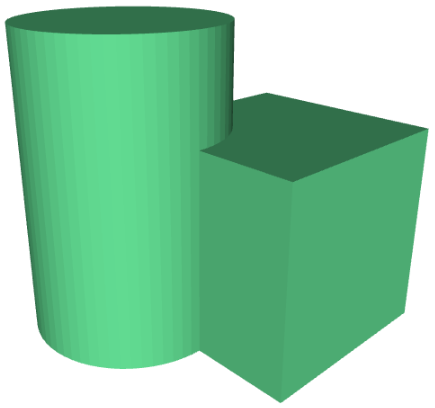
\includegraphics[width=0.35\textwidth]{img/diff-0.png}
\end{center}
\vspace{-4mm}
\caption{Displaying the two objects.}
\label{fig:diff-0}
%\vspace{-1cm}
\end{figure}
\noindent
Now let's subtract the cylinder from the cube -- just replace 
{\tt STRUCT} with {\tt DIFF}:

\begin{bluecode}
out = DIFF(c, s) 
\end{bluecode}
\index{DIFF}
The output is shown in Fig. \ref{fig:diff-1}.
\newpage

\begin{figure}[!ht]
\begin{center}
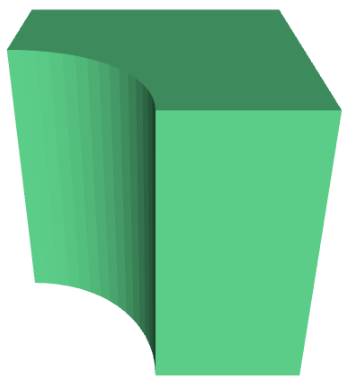
\includegraphics[width=0.25\textwidth]{img/diff-1.png}
\end{center}
\vspace{-4mm}
\caption{Subtracting the cylinder from the cube.}
\label{fig:diff-1}
%\vspace{-1cm}
\end{figure}
\noindent
We can also subtract the cube from the cylinder by switching 
the order of the arguments in the {\tt DIFF} command:

\begin{bluecode}
out = DIFF(s, c) 
\end{bluecode}
\index{DIFF}
The output is shown in Fig. \ref{fig:diff-2}.


\begin{figure}[!ht]
\begin{center}
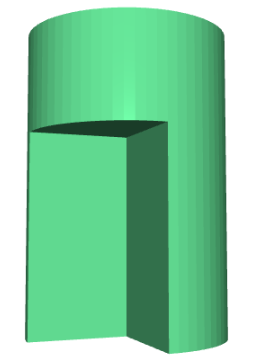
\includegraphics[width=0.23\textwidth]{img/diff-2.png}
\end{center}
\vspace{-4mm}
\caption{Subtracting the cube from the cylinder.}
\label{fig:diff-2}
%\vspace{-1cm}
\end{figure}
\noindent
PLaSM makes it possible to subtract multiple objects from an 
object, by using  the {\tt DIFF} command with more then two arguments.
Then the second, third, fourth, etc. objects are subtracted
from the first one. For illustration, let is create a cube and
three cylinders:

\begin{bluecode}
c = CUBE(2.0)
s = CYLINDER(1.0, 3.0)
s2 = R(s, 1, -PI/2)
s3 = R(s, 2, -PI/2)
out = STRUCT(c, s, s2, s3) 
\end{bluecode}
\index{CUBE}
\index{CYLINDER}
\index{ROTATE}
\index{STRUCT}
The output is shown in Fig. \ref{fig:diff-3}.
\newpage

\begin{figure}[!ht]
\begin{center}
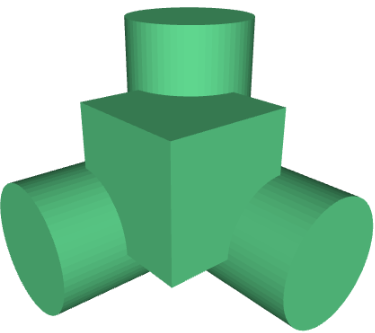
\includegraphics[width=0.45\textwidth]{img/diff-3.png}
\end{center}
\vspace{-4mm}
\caption{Displaying the four objects.}
\label{fig:diff-3}
%\vspace{-1cm}
\end{figure}
\noindent
Changing {\tt STRUCT} to {\tt DIFF} in the above script

\begin{bluecode}
out = DIFF(c, s, s2, s3) 
\end{bluecode}
\index{DIFF}
subtracts the cylinders from the cube, as shown in Fig. \ref{fig:diff-4}.

\begin{figure}[!ht]
\begin{center}
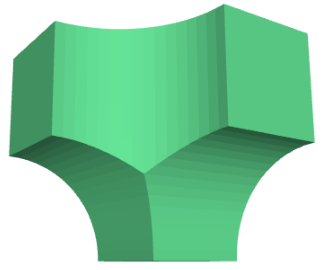
\includegraphics[width=0.35\textwidth]{img/diff-4b.png}
\end{center}
\vspace{-4mm}
\caption{Resulting object: cube minus three cylinders.}
\label{fig:diff-4}
%\vspace{-1cm}
\end{figure}

\subsection{Creating union of objects}\label{subsec:union}

The {\tt UNION} command (that can be abbreviated as {\tt U})
creates a new object that is the set union 
of two or more objects. Although the result of {\tt UNION}
is visually identical to the result of {\tt STRUCT}, 
there is a huge difference between the two commands.
The {\tt STRUCT} command does not create a new object, it just 
groups existing objects for visualization (or other)  purposes. 
The {\tt UNION} command creates a new 
object that can be used for further manipulation. Let us 
illustrate this by using the four objects from the last 
example. 

\begin{bluecode}
c = CUBE(2.0)
s = CYLINDER(1.0, 3.0)
s2 = R(s, 1, -PI/2)
s3 = R(s, 2, -PI/2)
out = U(c, s, s2, s3) 
\end{bluecode}
\index{CUBE}
\index{CYLINDER}
\index{ROTATE}
\index{UNION}
The output is shown in Fig. \ref{fig:union}.\\

%\newpage

\begin{figure}[!ht]
\begin{center}
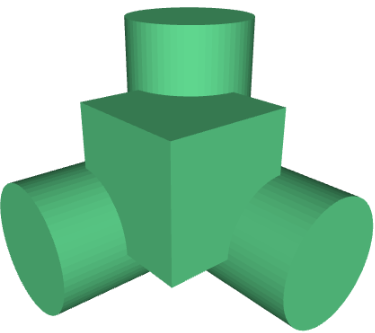
\includegraphics[width=0.35\textwidth]{img/diff-3.png}
\end{center}
\vspace{-4mm}
\caption{Union of the three cylinders and the cube.}
\label{fig:union}
%\vspace{-1cm}
\end{figure}


\subsection{Creating intersection of objects}\label{subsec:intersection}

PLaSM performs intersections using the {\tt INTERSECTION} command (that can be 
abbreviated as {\tt I}). We will show two examples. First we will create the 
intersection of the cube and the three cylinders from the last example:
 
\begin{bluecode}
c = CUBE(2.0)
s = CYLINDER(1.0, 3.0)
s2 = R(s, 1, -PI/2)
s3 = R(s, 2, -PI/2)
out = I(c, s, s2, s3) 
\end{bluecode}
\index{CUBE}
\index{CYLINDER}
\index{ROTATE}
\index{INTERSECTION}
The output is shown in Fig. \ref{fig:int-2}.


\begin{figure}[!ht]
\begin{center}
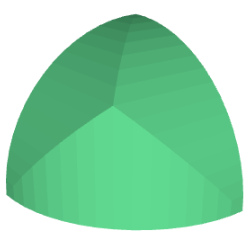
\includegraphics[width=0.2\textwidth]{img/int-2a.png}\ \ \ 

\includegraphics[width=0.2\textwidth]{img/int-2b.png}
\end{center}
\vspace{-4mm}
\caption{Intersection of the three cylinders and the cube (two different views).}
\label{fig:int-2}
%\vspace{-1cm}
\end{figure}
\noindent
Next let us create 
a strange object that looks like a square from one side,
circle from another side, and triangle the third direction. 
Here is the script,

\begin{bluecode}
c = CUBE(2.0)
c = T(c, -1, -1, -1)
cyl = CYLINDER(1, 2)
cyl = T(cyl, 0, 0, -1)
p = CONVEXHULL([1, -1, -1], [1, 0, 1], [1, 1, -1], \
                [-1, -1, -1], [-1, 0, 1], [-1, 1, -1])
out = I(c, cyl, p)
\end{bluecode}
\index{CUBE}
\index{TRANSLATE}
\index{CYLINDER}
\index{CONVEXHULL}
\index{INTERSECTION}
and its output is shown in Fig. \ref{fig:diff-1}.\\

\begin{figure}[!ht]
\begin{center}

\includegraphics[width=0.25\textwidth]{img/int-1a.png}
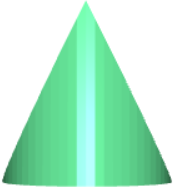
\includegraphics[width=0.25\textwidth]{img/int-1b.png}

\includegraphics[width=0.25\textwidth]{img/int-1c.png}
\end{center}
\vspace{-4mm}
\caption{What a strange object!}
\label{fig:int-1}
%\vspace{-1cm}
\end{figure}


\subsection{Creating XOR of objects}\label{subsec:xor}

The operation XOR a.k.a. "union minus intersection" can be illustrated  
on an example where a cube is moved so that it's center lies on the $z$-axis. Then 
a second cube is created by rotating the original one by 45 degrees about the 
$x$-axis. Last, the two cubes are XORred:
 
\begin{bluecode}
c = CUBE(2.0)
c = T(c, -1, -1, 0)
c2 = R(c, 3, PI/4)
out = XOR(c, c2) 
\end{bluecode}
\index{CUBE}
\index{TRANSLATE}
\index{ROTATE}
\index{XOR}
The output is shown in Fig. \ref{fig:xor-1}.
\newpage

\begin{figure}[!ht]
\begin{center}
\includegraphics[width=0.35\textwidth]{img/xor-new1a.png}\ \ \ \ \ \ \ 
\includegraphics[width=0.35\textwidth]{img/xor-new.png}
\end{center}
\vspace{-4mm}
\caption{Union (left) and XOR (right) of two overlapping cubes.}
\label{fig:xor-1}
%\vspace{-1cm}
\end{figure}
\noindent
Again, it is possible to XOR multiple objects by passing all of them 
into the {\tt XOR} command.

\subsection{Doing it the wrong way, doing it the right way}

Boolean operations can lead to unnecessarily long computations if not done 
properly. They should be as much {\em local} as possible, meaning that 
they should occur between as {\em geometrically simple objects} as possible.

We will demonstrate this on an example where we first create a vault and then play 
a gangster and drill a hole into it. Do not worry about the lenght of the script below  because
the vault has many small parts. But the fact that there are many parts is important here.
We will show that while performing a Boolean operation between the drill and the entire
vault is extremely time consuming, drilling just into just the one relevant part
of the geometry is done quickly.

The model is available as Displayed Project "PLaSM - Examples - Vault". First, let us 
define the vault:

{\small
\begin{bluecode}
# Define main vault body:
body = BRICK(1, 1, 1.2)
interior = BRICK(0.86, 0.95, 1.06)
interior = T(interior, 0.07, 0, 0.07)
body = DIFF(body, interior)

# Top part:
top = CONVEXHULL([0, 0, 1.2], [1, 0, 1.2], [1, 1, 1.2], [0, 1, 1.2], [0.01, 0.01, 1.21], \
                 [0.99, 0.01, 1.21], [0.99, 0.99, 1.21], [0.01, 0.99, 1.12])

# Shelves:
shelf = BRICK(1, 0.85, 0.02)
shelf1 = T(shelf, 0, 0.1, 0.4)
shelf2 = T(shelf1, 0, 0, 0.4)

# Front door:
door = BRICK(0.84, 0.05, 1.04)
door = T(door, 0.08, 0, 0.08)
door_frame = BRICK(0.86, 0.03, 1.06)
door_frame = T(door_frame0.07, 0.02, 0.07)

# Truncated cone under the handles:
tcone = TRUNCONE(0.14, 0.13, 0.02)
tcone = R(tcone, 1, PI/2)
tcone = T(tcone, 0.5, 0, 0.6)

# Cylinder that holds the handles:
cyl = CYLINDER(0.07, 0.1)
cyl = R(cyl, 1, PI/2)
cyl = T(cyl, 0.5, 0, 0.6)

# Small truncated cone at the handles:
stcone = TRUNCONE(0.07, 0.06, 0.01)
stcone = R(stcone, 1, PI/2)
stcone = T(stcone, 0.5, -0.1, 0.6)

# Handles:
h1 = CYLINDER(0.022, 0.3)
ts = TRUNCONE(0.022, 0.017, 0.01)
ts = T(ts, 0, 0, 0.3)
h1 = U(h1, ts)
h1 = R(h1, 1, PI/24)
h1 = R(h1, 2, -7*PI/24)
h2 = R(h1, 2, -2*PI/3)
h3 = R(h2, 2, -2*PI/3)
h1 = T(h1, 0.5, -0.06, 0.6)
h2 = T(h2, 0.5, -0.06, 0.6)
h3 = T(h3, 0.5, -0.06, 0.6)

# Bolts:
b1 = CONVEXHULL([0.81, 0, 0.19], [0.83, 0, 0.17], [0.97, 0, 0.17], [0.97, 0, 0.26], \
                [0.83, 0, 0.26], [0.81, 0, 0.24], [0.815, -0.01, 0.195], [0.835, -0.01, 0.175], \
                [0.965, -0.01, 0.175], [0.965, -0.01, 0.255], [0.835, -0.01, 0.255], [0.815, -0.01, 0.235])
b2 = T(b1, 0, 0, 0.77)

# Bolt cylinder:
bc = CYLINDER(0.015, 0.1, 16)
bc1 = T(bc, 0.925, -0.009, 0.165)
bc2 = T(bc1, 0, 0, 0.77)

# Small bolt sphere:
sbc = SPHERE(0.01, [8, 8])
sbc = R(sbc, 1, PI/2)
sbc1 = T(sbc, 0.845, -0.01, 0.195)
sbc2 = T(sbc1, 0, 0, 0.035)
sbc3 = T(sbc1, 0, 0, 0.77)
sbc4 = T(sbc3, 0, 0, 0.035)

# Vertical handle:
vh = CYLINDER(0.02, 0.5, 16)
vh = T(vh, 0.15, -0.04, 0.35)

# Vertical handle supports:
vh0 = CYLINDER(0.015, 0.06, 16)
vh0 = R(vh0, 1, PI/2)
vh0 = T(vh0, 0.15, 0.02, 0.4)
vh1 = T(vh0, 0, 0, 0.4)

# Put everything together:
rest = STRUCT(top, shelf1, shelf2, door, door_frame, tcone, cyl, stcone, h1, h2, h3, b1, \
              b2, bc1, bc2, sbc1, sbc2, sbc3, sbc4, vh, vh0, vh1)
vault = STRUCT(body, rest)
lab.view(vault)
\end{bluecode}
}
\index{BRICK}
\index{TRANSLATE}
\index{DIFF}
\index{CONVEXHULL}
\index{ROTATE}
\index{CYLINDER}
\index{TRUNCONE}
\index{UNION}
\index{SPHERE}
\index{STRUCT}
\noindent
The output is shown in Fig.\ref{fig:vault}.\\

\begin{figure}[!ht]
\begin{center}
\includegraphics[width=0.4\textwidth]{img/vault.png}
\end{center}
\vspace{-4mm}
\caption{Vault model.}
\label{fig:vault}
%\vspace{-1cm}
\end{figure}
\noindent
Now let's define the drill: 
\begin{bluecode}
drill = CYLINDER(0.1, 0.5)
drill = R(drill, 2, PI/2)
drill = T(drill, 0.1, 0.5, 0.55)
\end{bluecode}
\index{CYLINDER}
\index{ROTATE}
\index{TRANSLATE}
\index{}Now let's drill into the vault. First we will do it 
the wrong way -- drilling into the {\tt vault} object
that consists of many parts. 

\begin{bluecode}
drilled_vault = DIFF(vault, drill)
lab.view(STRUCT(drilled_vault))
\end{bluecode}
\index{DIFF}
\index{STRUCT}
You can run this script but it will take a long time.

The correct way is to perform the Boolean 
operation between the {\tt drill} and the {\tt body} 
because the {\tt body} object that is much simpler 
than the complete {\tt vault}: 

\begin{bluecode}
drilled_body = DIFF(body, drill)
lab.view(STRUCT(drilled_body, rest))
\end{bluecode}
\index{DIFF}
\index{STRUCT}
Now the computation takes just a few milliseconds!
The output is shown in Fig.\ref{fig:vault2}.

\begin{figure}[!ht]
\begin{center}
\includegraphics[width=0.4\textwidth]{img/vault2.png}
\end{center}
\vspace{-4mm}
\caption{Vault is drilled, and money is gone!}
\label{fig:vault2}
\end{figure}
\noindent




\section{Curves and Curved Surfaces}\label{sec:curves}

\subsection{Objectives}
\begin{itemize}
\item Understand the concept of reference domains and reference maps.
\item Learn to map curves and surfaces in 3D space.
\item Understand B\'ezier curves.
\item Create B\'ezier curves and surfaces.
\item Create coons patches.
\item Create rotational surfaces.
\item Learn how to solidify a surface.
\item Create ruled surfaces.
\item Learn to span surfaces between curves.
\item Create cylindrical and conical surfaces.
\item Create profile product surfaces.
\item Create cubic Hermite surfaces.
\end{itemize}
PLaSM provides extensive support for curved surfaces including 
B\'ezier surfaces, coons patches, rotational surfaces, ruled surfaces,  
cylindrical and conical surfaces, Hermite surfaces, 
splines, Cartesian products of curves, etc. These techniques will be 
discussed in the following, but first let us explain the underlying 
concepts of {\em reference domains} and {\em maps}.

\subsection{Reference domains}

In a standard way, curves in PLaSM are parameterized from an interval,
and surfaces from a rectangle. These domains are called
{\em reference domains}. 

Reference interval $(0, L)$ that is subdivided into $N$ equally-long pieces is 
created using the command {\tt INTERVALS}:

\begin{bluecode}
ref_domain = INTERVALS(L, N)
\end{bluecode}
\index{INTERVALS}
Reference rectangle $(0, L_1) \times (0, L_2)$, where the first and second 
directions are subdivided into $N_1$ and $N_2$ pieces, respectively, can be 
created using the {\tt POWER} command:

\begin{bluecode}
dom1 = INTERVALS(L1, N1)
dom2 = INTERVALS(L2, N2)
ref_domain = POWER(dom1, dom2)
\end{bluecode}
\index{INTERVALS}

\subsection{Mapping curves}

Every curve is the graph of a {\em function} $P$ that is defined 
in a reference interval $(0, L)$ and for every value $t$ in this 
interval it returns a 3D point $P(t)$. The function 
$P$ is called {\em reference map}. Let us show a few examples.\\

\noindent
\underline{\em Example 1}: The map

$$
P(t) = [1+t, 1+t, 1+t]
$$
which in Python is written as

\begin{bluecode}
def P(t):
    return [1 + t, 1 + t, 1 + t]
\end{bluecode}
renders for $t$ in $(0, 1)$ a curve that is a straight line connecting the 
points (1, 1, 1) and (2, 2, 2), as shown in Fig. \ref{fig:paramcu1}.
\newpage

\begin{figure}[!ht]
\begin{center}
\includegraphics[width=0.4\textwidth]{img/paramcu1.png}
\end{center}
\vspace{-6mm}
\caption{Graph of the reference map $P(t) = [1+t, 1+t, 1+t]$.}
%\vspace{-1cm}
\label{fig:paramcu1}
\end{figure}
\noindent
How can we verify that this graph is correct? 
Insert the limit values $t = 0$ and $t = 1$ into the formula for the map $P$ 
to see that the end points are (1, 1, 1) and (2, 2, 2), respectively. The 
fact that the curve is a straight line follows from the linearity of the 
map $P$ in all three components. \\

\noindent
\underline{\em Example 2}: The map

$$
P(t) = [\cos(t), \sin(t), 0]
$$
whose Python form is

\begin{bluecode}
def P(t):
    return [cos(t), sin(t), 0]
\end{bluecode}
maps the reference interval $(0, 2\pi)$ to a circle in the 
$xy$-plane, as shown in Fig. \ref{fig:paramcu2}.

\begin{figure}[!ht]
\begin{center}
\includegraphics[width=0.4\textwidth]{img/paramcu2.png}
\end{center}
\vspace{-6mm}
\caption{Graph of the reference map $P(t) = [\cos(t), \sin(t), 0]$.}
\label{fig:paramcu2}
\end{figure}
\noindent
\newpage
\noindent
\underline{\em Example 3}: The map

$$
P(t) = [0, \cos(t), \sin(t)]
$$
a.k.a.

\begin{bluecode}
def P(t):
    return [0, cos(t), sin(t)]
\end{bluecode}
maps the reference interval $(0, 2\pi)$ to a circle in the 
$yz$-plane, as shown in Fig. \ref{fig:paramcu3}.

\begin{figure}[!ht]
\begin{center}
\includegraphics[width=0.4\textwidth]{img/paramcu3.png}
\end{center}
\vspace{-6mm}
\caption{Graph of the reference map $P(t) = [0, \cos(t), \sin(t)]$.}
\label{fig:paramcu3}
\end{figure}
\noindent
\underline{\em Example 4}: The map

$$
P(t) = [\cos(t), \sin(t), t]
$$
or

\begin{bluecode}
def map(t):
    return [cos(t), sin(t), t]
\end{bluecode}
maps the reference interval $(0, 2\pi)$ to a spiral whose 
$xy$-plane projection is the unit circle and in the $z$-direction 
spans the interval $(0, 2\pi)$, as shown in Fig. \ref{fig:paramcu4}.
\newpage

\begin{figure}[!ht]
\begin{center}
\includegraphics[width=0.4\textwidth]{img/paramcu4.png}
\end{center}
\vspace{-6mm}
\caption{Graph of the reference map $P(t) = [\cos(t), \sin(t), t]$.}
\label{fig:paramcu4}
\end{figure}
\noindent

\subsection{Mapping surfaces}

Now that the reader understands the parameterization of curves, surfaces will 
follow easily. In fact the only difference is that the reference map 
$P(t_1, t_2)$ is a function of two variables -- it still returns 3D points. 
Let us show a few examples.\\

\noindent
\underline{\em Example 1}: The map

$$
P(t_1, t_2) = [t_1, t_2, t_1 + t_2]
$$
\noindent
whose code is

\begin{bluecode}
def P(t1, t2):
    return [t1, t2, t1 + t2]
\end{bluecode}
maps the reference square $(0, 1)\times(0, 1)$ to a planar surface that spans
four points (0, 0, 0), (1, 0, 1), (0, 1, 1) and (1, 1, 2). No subdivision in
any direction was applied to the reference square to generate the wireframe plot 
shown in Fig. \ref{fig:paramsu1}. In other words, only the four vertices of the reference domain 
were transformed using the map, and the resulting 3D points were interpolated
linearly. This was enough in this case since the resulting surface is linear.
\newpage

\begin{figure}[!ht]
\begin{center}
\includegraphics[width=0.4\textwidth]{img/paramsu1.png}
\end{center}
\vspace{-6mm}
\caption{Graph of the reference map $P(t_1, t_2) = [t_1, t_2, t_1 + t_2]$.}
\label{fig:paramsu1}
\end{figure}
\noindent

\noindent
\underline{\em Example 2}: Next we render a saddle surface
using the reference square $(-1, 1)\times(-1, 1)$. 
The map is defined as

$$
P(t_1, t_2) = [t_1, t_2, t_1 t_2]
$$
or

\begin{bluecode}
def P(t1, t2):
    return [t1, t2, t1*t2]
\end{bluecode}
The reference square was subdivided into $10$ intervals in each direction, i.e., into 
100 square cells. This means that $11^2$ points were transformed via the map $P(t_1, t_2)$.
The corresponding wireframe plot with 100 linearly interpolated cells is shown in Fig. \ref{fig:paramsu1c}. 

\begin{figure}[!ht]
\begin{center}
\includegraphics[width=0.4\textwidth]{img/paramsu1c.png}
\end{center}
\vspace{-6mm}
\caption{Graph of the reference map $P(t_1, t_2) = [t_1, t_2, t_1 t_2]$.}
\label{fig:paramsu1c}
\end{figure}
\noindent
\noindent
\underline{\em Example 3}: Now let us render a cylindrical surface 
of radius 1 and height 1 using the reference rectangle $(0, 2\pi)\times(0, 1)$. 
The interval $(0, 2\pi)$ represents angular direction and $(0, 1)$ the $z$-direction. 
The map is defined as

$$
P(a, z) = [\cos(a), \sin(a), z]
$$
or

\begin{bluecode}
def P(a, z):
    return [cos(a), sin(a), z]
\end{bluecode}
The reference domain was subdivided into 32 equally-long subintervals in the angular direction,
and it was not subdivided in the $z$-direction. Hence the wireframe plot shown in 
Fig. \ref{fig:paramsu20} consists of 32 linear surfaces. 

\begin{figure}[!ht]
\begin{center}
\includegraphics[width=0.4\textwidth]{img/paramsu20.png}
\end{center}
\vspace{-6mm}
\caption{Graph of the reference map $P(a, z) = [\cos(a), \sin(a), z]$.}
\label{fig:paramsu20}
\end{figure}
\noindent
In fact, PLaSM uses the same map to render cylindrical surfaces, and that's
is where the optional subdivision parameter in the {\tt CYLINDER} command comes from.
In PLaSM, its default value is 64. 

\subsection{Three ways to map a sphere}

Usually there is more than one way to 
map a given surface. The maps will differ in their properties 
and some of them will be better than the others. Let us
illustrate this using the spherical surface as an example. 
\newpage

\noindent
\underline{\em Map 1}: Let us begin with the simplest map based on parameterizing 
the angular and radial directions. The reference rectangle is $(0, 2\pi)\times(0, 1)$. 
where $(0, 2\pi)$ represents the angle and $(0, 1)$ the radius. The map is given by the formula

$$
P(a, r) = \left[r\cos(a), r\sin(a), \sqrt{1 - r^2}\right]
$$
or

\begin{bluecode}
def P(a, r):
    return [r*cos(a), r*sin(a), sqrt(1 - r**2)]
\end{bluecode}
We subdivide the reference rectangle into 32 pieces in the angular direction
and into 10 pieces in the radial one. This means that the piecewise linear 
wireframe plot shown in Fig. \ref{fig:paramsu5} has 320 cells. \\

\begin{figure}[!ht]
\begin{center}
\includegraphics[width=0.4\textwidth]{img/paramsu5.png}
\end{center}
\vspace{-6mm}
\caption{Graph of the reference map $P(a, r) = \left[r\cos(a), r\sin(a), \sqrt{1 - r^2}\right]$.}
\label{fig:paramsu5}
\end{figure}
\noindent
Notice that many points are accumulated near the pole while the lower portion
of the surface is approximated rather crudely. \\

\noindent
\underline{\em Map 2}: This map uses the angle and the $z$-direction. The 
reference rectangle is formally the same as before, $(0, 2\pi)\times(0, 1)$,
but the interval $(0, 1)$ has a different meaning. Also the map is different,

$$
P(a, z) = \left[\sqrt{1 - z^2}\cos(a), \sqrt{1 - z^2}\sin(a), z\right]
$$
or

\begin{bluecode}
def P(a, z):
    return [sqrt(1 - z**2)*cos(a), sqrt(1 - z**2)*sin(a), z]
\end{bluecode}
The wireframe plot shown in Fig. \ref{fig:paramsu3} is based on precisely the 
same subdivision of the reference rectangle as in the previous case. 

\begin{figure}[!ht]
\begin{center}
\includegraphics[width=0.45\textwidth]{img/paramsu6.png}
\end{center}
\vspace{-6mm}
\caption{Graph of the reference map $P(a, z) = \left[\sqrt{1 - z^2}\cos(a), \sqrt{1 - z^2}\sin(a), z\right]$.}
\label{fig:paramsu3}
\end{figure}
\noindent
The reader can see that while the lower portion of the surface is approximated 
better compared to the previous case, the accuracy suffers in the vicinity of the pole.\\

\noindent
\underline{\em Map 3}: The last map uses two angular directions $a$ and $b$ and 
a different reference rectangle $(0, 2\pi)\times(0, \pi/2)$. The map is 
defined as

$$
P(a, b) = \left[\cos(a)\cos(b), \sin(a)\cos(b), \sin(b)\right]
$$
or

\begin{bluecode}
def P(a, z):
    return [cos(a)*cos(b), sin(a)*cos(b), sin(b)]
\end{bluecode}
The wireframe plot shown in Fig. \ref{fig:paramsu8} is also based on a
$32 \times 10$ subdivision of the reference rectangle which results into the 
same number of 320 linear cells that we had in the previous two examples.
However, the reader can see that this map yields clearly the best approximation. 

\begin{figure}[!ht]
\begin{center}
\includegraphics[width=0.4\textwidth]{img/paramsu8.png}
\end{center}
\vspace{-6mm}
\caption{Graph of the reference map $P(a, b) = \left[\cos(a)\cos(b), \sin(a)\cos(b), \sin(b)\right]$.}
\label{fig:paramsu8}
\end{figure}
\noindent
Therefore PLaSM uses precisely this map to 
render spherical surfaces. In fact PLaSM uses a reference rectangle $(0, 2\pi)\times(-\pi/2, \pi/2)$
to cover the entire sphere. The default subdivision for the spherical surface in PLaSM
is $48 \times 24$ which corresponds to

\begin{bluecode}
s = SPHERE(R, [24, 48])
\end{bluecode}
\index{SPHERE}
(the order of the two subdivisions is switched).
\subsection{Primer on B\'ezier curves}

B\'ezier curves are the most widely used curves in engineering design. 
Let us begin with the linear case. Linear B\'ezier curve is a straight line that
connects two control points $P_1$ and $P_2$. All B\'ezier curves are parameterized
from the interval $[0, 1]$, so in the linear case the exact mathematical definition is
$$
  B(t) = P_1 + t(P_2 - P_1)
$$ 
You can easily check that the curve starts at $P_1$ (substitute $t = 0$ to the above formula),
and that it ends at $P_2$ (substitute there $t = 1$).

Quadratic B\'ezier curves are defined using three control points $P_1, P_2$ and $P_3$. Again they are
parameterized from $[0, 1]$, and their definition is

$$
  B(t) = (1 - t)^2 P_1 + 2(1 - t)t P_2 + t^2 P_3.
$$ 
Cubic B\'ezier curves are defined using four control points $P_1, P_2, P_3$ and $P_4$. They are
parameterized from $[0, 1]$ as usual, and their definition is

$$
  B(t) = (1 - t)^3 P_1 + 3(1 - t)^2t P_2 + 3(1-t)t^2 P_3 + t^3 P_4.
$$ 

\subsection{Surface with one curved B\'ezier edge}

To begin with, let us create a 2D quadrilateral that has one cubic B\'ezier edge. 
B\'ezier curves are created using the commands {\tt BEZIER\_1} and {\tt BEZIER\_2} 
(that can be abbreviated as {\tt BE\_1} and {\tt BE\_2}). The difference between
them is in how they are mapped on the reference domain. The former use the 
first coordinate of domain points, the latter use the second coordinate. Let
us create two curves, one linear and one cubic:

\begin{bluecode}
# Linear Bezier curve:
c1 = BEZIER_1([0, 0, 0], [0, 4, 0])

# Cubic Bezier curve:
c2 = BEZIER_1([2, 0, 0], [4, 1, 0], [0, 2, 0], [1, 3, 0])
\end{bluecode}
\index{BEZIER\_1}
\noindent
The surface between these two curves needs to be treated as any other curved 
surface and thus it needs to be mapped on a reference rectangle. For simplicity 
(applies generally), we may use the unit square. 

\begin{bluecode}
# Reference domain with 30 times 30 subdivision:
ref_domain = UNIT_SQUARE(30, 30)

# The 2D surface:
surf = BEZIER_2(c1, c2)
out = MAP(ref_domain, surf)
\end{bluecode}
\index{UNIT\_SQUARE}
\index{BEZIER\_2}
\index{MAP}
The output is displayed in Fig. \ref{fig:curves-1}.\\

\begin{figure}[!ht]
\begin{center}
\includegraphics[width=0.3\textwidth]{img/curves-1.png}
\end{center}
\vspace{-4mm}
\caption{Surface with one curved B\'ezier edge.}
\label{fig:curves-1}
%\vspace{-1cm}
\end{figure}

\noindent
Remarks:
\begin{itemize}
\item As we already saw in a different context before, a point list
such as {\tt L = [[0, 0, 0], [0, 4, 0]]} can be passed into 
the {\tt BEZIER\_1} and {\tt BEZIER\_2} functions as well, with 
an asterisk in front of it, i.e., as {\tt BEZIER\_1(*L)} or {\tt BEZIER\_2(*L)}.
\item Notice that the commands accepts general 3D points, they do not have 
to lie in the $xy$-plane as they are in this example.
\end{itemize}

\subsection{Surface with two curved B\'ezier edges}

This example is very similar to the last one, and we are showing it 
only to illustrate that both the B\'ezier edges can be curves. 
Concretely, the curve {\tt c1} is made parabolic by adding one 
more control point to it. 

\begin{bluecode}
# Quadratic Bezier curve:
c1 = BEZIER_1([0, 0, 0], [-1, 1.5, 0], [0, 4, 0])

# Cubic Bezier curve:
c2 = BEZIER_1([2, 0, 0], [4, 1, 0], [0, 2, 0], [1, 3, 0])

# Reference domain with 30 times 30 subdivision:
ref_domain = UNIT_SQUARE(30, 30)

# The 2D surface:
surf = BEZIER_2(c1, c2)
out = MAP(ref_domain, surf)
\end{bluecode}
\index{BEZIER\_1}
\index{BEZIER\_2}
\index{UNIT\_SQUARE}
\index{MAP}

The output is displayed in Fig. \ref{fig:curves-2}.

\begin{figure}[!ht]
\begin{center}
\includegraphics[width=0.36\textwidth]{img/curves-2.png}
\end{center}
\vspace{-4mm}
\caption{Surface with two curved B\'ezier edges.}
\label{fig:curves-2}
%\vspace{-1cm}
\end{figure}

\subsection{Surface with four curved B\'ezier edges}

Next let us construct a B\'ezier surface spanning four 
B\'ezier edges. 

\begin{bluecode}
# Bezier curves:
c1 = BEZIER_1([0,0,0], [5, -2, -5], [10,0,0])
c2 = BEZIER_1([0,2,0], [8,3,0], [9,2,0])
c3 = BEZIER_1([0,4,1], [7,5,-1], [8,5,1], [12,4,0])
c4 = BEZIER_1([0,6,0], [9,6,3], [10,6,-1])

# Reference domain with 30 times 30 subdivision:
ref_domain = UNIT_SQUARE(30, 30)

# The surface:
surf = BEZIER_2(c1, c2, c3, c4)
out = MAP(ref_domain, surf)
\end{bluecode}
\index{BEZIER\_1}
\index{UNIT\_SQUARE}
\index{BEZIER\_2}
\index{MAP}
The output is displayed in Fig. \ref{fig:bezi}.

\begin{figure}[!ht]
\begin{center}
\includegraphics[width=0.5\textwidth]{img/bezi.png}
\end{center}
\vspace{-4mm}
\caption{Surface with four curved B\'ezier edges.}
\label{fig:bezi}
%\vspace{-1cm}
\end{figure}

\subsection{Coons patch}

{\em Coons patch} is a technique that forms a B\'ezier patch from four B\'ezier edges connected 
by their end points. The center control 
points are calculated by a blend of two linear interpolations and one bilinear interpolation.

\begin{bluecode}
u1 = BEZIER_1([0, 4, 0], [2.5, 3, 6], [5, 0, -6], [7.5, 0, 6], [10, 0, 0])
u2 = BEZIER_1([0, 6, 0], [2.5, 7, 6], [5, 10, -6], [7.5, 10, 6], [10, 10, 0])
v1 = BEZIER_2([0, 0, 0], [-3, 3, 3], [-3, 7, 3], [0, 10, 0])
v2 = BEZIER_2([10, 0, 0], [15, 6, 0], [10, 10, 0])

# Reference domain:
ref_domain = UNIT_SQUARE(50, 50)

# The cons patch:
surf = COONSPATCH(u1, u2, v1, v2)
out = MAP(ref_domain, surf)
\end{bluecode}
\index{BEZIER\_1}
\index{BEZIER\_2}
\index{UNIT\_SQUARE}
\index{COONSPATCH}
\index{MAP}
The output is displayed in Fig. \ref{fig:curves-3}.
\newpage

\begin{figure}[!ht]
\begin{center}
\includegraphics[width=0.5\textwidth]{img/curves-3.png}
\end{center}
\vspace{-4mm}
\caption{Coons patch.}
\label{fig:curves-3}
%\vspace{-1cm}
\end{figure}

\subsection{Rotational surface}

Rotational surfaces can be created using the {\tt ROTATIONAL\_SURFACE} command
(possibly abbreviated as {\tt ROSURFACE} or {\tt ROS}).
The rotation is done about the $z$-axis. To achieve best results, the curve
should therefore be defined in a plane that contains the $z$-axis, and moreover 
it should entirely lie on one side of the $z$-axis without intersecting it.

\begin{bluecode}
# Sample Bezier profile in the xz-plane: 
parabola = BEZIER_1([0, 0, 0], [2, 0, 0], [3, 0, 4])
  
# Reference domain with 2*PI for angle:
ref_domain = REF_DOMAIN(1, 2*PI, 32, 64)

# Rotate about the z-axis:
surf = ROTATIONAL_SURFACE(parabola)
out = MAP(ref_domain, surf)
\end{bluecode}
\index{BEZIER\_1}
\index{REF\_DOMAIN}
\index{ROTATIONAL\_SURFACE}
\index{MAP}
The output is displayed in Fig. \ref{fig:curves-4}.\\

\begin{figure}[!ht]
\begin{center}
\includegraphics[width=0.35\textwidth]{img/curves-4.png}
\end{center}
\vspace{-4mm}
\caption{Rotational surface created using a quadratic B\'ezier curve.}
\label{fig:curves-4}
\vspace{-1cm}
\end{figure}
\newpage

\subsection{Solidifying a surface}

Surfaces can be solidified using the command {\tt JOIN}. The 
result of this operation will always be a convex hull. 
Adding to the last script:

\begin{bluecode}
# Solidify the surface:
out = JOIN(out)
\end{bluecode}
\index{JOIN}
This operation may take a while since PLaSM creates a new 
set of volume maps from the existing set of surface maps. 
The output is displayed in Fig. \ref{fig:curves-5}.\\

\begin{figure}[!ht]
\begin{center}
\includegraphics[width=0.35\textwidth]{img/curves-5.png}
\end{center}
\vspace{-4mm}
\caption{Solidifying surface from Fig. \ref{fig:curves-4}.}
\label{fig:curves-5}
%\vspace{-1cm}
\end{figure}


\subsection{Ruled surface - introduction}

In geometry, a surface $S$ is called {\em ruled} (or {\em scroll}) if it is "formed by straight lines".
More precisely, if through every point of $S$ passes a straight line that lies in $S$. 
The most familiar examples are the plane, cylinder, and 
cone. The standard definition of the ruled surface is 

$$
S(x, y) = p(x, y) + yq(x, y)
$$
where $p(x, y) = p(x)$ and $q(x, y) = q(x)$ are maps defined in a reference rectangle 
$A \times B$. None of them depends on the $y$-coordinate, just on $x$. For every $x$ in 
$A$, $p(x, y) = p(x)$ returns a 3D point on the surface $S$. The map $q(x, y) = q(x)$ returns 
for every $x$ in $A$ a direction vector (in the form of a 3D point). This is the direction 
of the straight line that lies on the surface $S$. The values of $y$ are in the interval $B$.

In the first example, the map $p(x, y) = p(x)$ is defined as

$$
p(x, y) = (x, 0, 0)
$$
and thus the curve lying on $S$ is a straight line connecting the points 
(0, 0, 0) and (1, 0, 0). 

\begin{bluecode}
def p(point):
    x = point[0]
    return [x, 0, 0]
\end{bluecode}
The map $q(x, y) = q(x)$ is given by

$$
q(x, y) = (0, 1, x).
$$
and it defines a direction vector that changes gradually from 
(0, 1, 0) to (0, 1, 1) as $x$ goes from 0 to 1.

\begin{bluecode}
def q(point):
    x = point[0]
    return [0, 1, x]
\end{bluecode}
Reference domain is the unit square covered with a $32 \times 32$
division:

\begin{bluecode}
# Unit square covered with a 32x32 Cartesian grid:  
ref_domain = UNIT_SQUARE(32, 32)
\end{bluecode}
\index{UNIT\_SQUARE}
The {\tt RULED\_SURFACE} command takes the two maps {\tt p, q}
as arguments. It can be abbreviated as {\tt RUSURFACE}: 

\begin{bluecode}
# Creating the ruled surface:
surf = RULED_SURFACE(p, q)
out = MAP(ref_domain, surf)
\end{bluecode}
\index{RULED\_SURFACE}
\index{MAP}
The output is displayed in Fig. \ref{fig:curves-6}.

\begin{figure}[!ht]
\begin{center}
\includegraphics[width=0.3\textwidth]{img/curves-6.png}
\end{center}
\vspace{-4mm}
\caption{Ruled surface given by the maps $p$ and $q$.}
\label{fig:curves-6}
%\vspace{-1cm}
\end{figure}

\subsection{Ruled surface - spiral}

In this example the map $p(x, y) = p(x)$ moves the 3D point 
along the $z$-axis and the direction vector $q(x, y) = q(x)$ 
is horizontal and rotates. The resulting surface $S$ is a spiral.

\begin{bluecode}
# Import sine and cosine from Numpy:
from numpy import sin, cos

def p(point):
    x = point[0]
    return [0, 0, 0.5*x]
  
def q(point):
    x = point[0]
    return [cos(x), sin(x), 0]

# Reference domain:  
ref_domain = REF_DOMAIN(8*PI, 5, 128, 16)

# Creating the ruled surface:
surf = RULED_SURFACE(p, q)
out = MAP(ref_domain, surf)
\end{bluecode}
\index{REF\_DOMAIN}
\index{RULED\_SURFACE}
\index{MAP}
The output is displayed in Fig. \ref{fig:curves-7}.\\

\begin{figure}[!ht]
\begin{center}
\includegraphics[width=0.3\textwidth]{img/curves-7.png}
\end{center}
\vspace{-4mm}
\caption{Spiral as a ruled surface.}
\label{fig:curves-7}
%\vspace{-1cm}
\end{figure}

\subsection{Ruled surface - straight cylinder}

In this example the map $p(x, y) = p(x)$ moves the 3D point on a circle 
that lies in the $xy$-plane, and the vector $q(x, y) = q(x)$ it a unit vector 
in the vertical direction. Hence the resulting ruled surface is a cylinder. 

\begin{bluecode}
# Import sine and cosine from Numpy:
from numpy import sin, cos

# Cylinder radius:
r = 3.0

# Cylinder height:
h = 10.0

def p(point):
    x = point[0]
    return [r*cos(x), r*sin(x), 0]
  
def q(point):
    x = point[0]
    return [0, 0, 1]

# Reference domain:  
ref_domain = REF_DOMAIN(2*PI, h, 64, 1)

# Creating the ruled surface:
surf = RULED_SURFACE(p, q)
out = MAP(ref_domain, surf)
\end{bluecode}
\index{REF\_DOMAIN}
\index{RULED\_SURFACE}
\index{MAP}
The output is displayed in Fig. \ref{fig:curves-8}.\\

\begin{figure}[!ht]
\begin{center}
\includegraphics[width=0.25\textwidth]{img/curves-8.png}
\end{center}
\vspace{-4mm}
\caption{Cylinder as a ruled surface.}
\label{fig:curves-8}
%\vspace{-1cm}
\end{figure}

\subsection{Ruled surface - curved cylinder}

This example is similar to the last one, except that the directional
vector $q(x, y) = q(x)$ is not vertical. Instead, it points 
to a point on the upper circle of the cylinder that has an 
angular shift $\alpha$. The script below uses a shift of $0.7\pi$. 
When increased towards $\pi$, the curved surface becomes thinner 
in the middle portion. 

\begin{bluecode}
# Import since and cosine from Numpy:
from numpy import sin, cos

# Cylinder radius:
r = 3.0

# Cylinder height:
h = 10.0

# Angular shift:
alpha = 0.7 * PI

def p(point):
    x = point[0]
    return [r*cos(x), r*sin(x), 0]
  
def q(point):
    x = point[0]
    return [r/h * (cos(x + alpha) - cos(x)), r/h * (sin(x + alpha) - sin(x)), 1]

# Reference domain::  
ref_domain = REF_DOMAIN(2*PI, h, 64, 32)

# Creating the ruled surface:
surf = RULED_SURFACE(p, q)
out = MAP(ref_domain, surf)
\end{bluecode}
\index{REF\_DOMAIN}
\index{RULED\_SURFACE}
\index{MAP}
The output is displayed in Fig. \ref{fig:curves-9}.\\

\begin{figure}[!ht]
\begin{center}
\includegraphics[width=0.25\textwidth]{img/curves-9.png}
\end{center}
\vspace{-4mm}
\caption{Curved cylinder.}
\label{fig:curves-9}
\vspace{-1cm}
\end{figure}
\newpage

\subsection{Ruled surface - spanning arbitrary 3D curves}

This is one of the most useful application of ruled surfaces.
We will show two examples. In the first one we consider 
a $2\pi \times 2\pi$ square, define a sine function and 
a parabola on the opposite edges, and connect them via 
a ruled surface:

\begin{bluecode}
# Import sine from Numpy:
from numpy import sin

# Define two 3D curves:
def c1(x):
    return [x, 0, sin(x)]

def c2(x):
    return [x, 2*PI, (x/PI - 1)**2]
  
def p(point):
    x = point[0]
    return c1(x)
  
# Return a vector pointing from one curve to the other:
def q(point):
    x = point[0]
    return [c2(x)[0] - c1(x)[0], c2(x)[1] - c1(x)[1], c2(x)[2] - c1(x)[2]]
  
# Reference domain:
ref_domain = REF_DOMAIN(2*PI, 1, 64, 1)

# Creating the ruled surface:
surf = RULED_SURFACE(p, q)
out = MAP(ref_domain, surf)
\end{bluecode}
\index{REF\_DOMAIN}
\index{RULED\_SURFACE}
\index{MAP}
The output is displayed in Fig. \ref{fig:curves-10}.\\

\begin{figure}[!ht]
\begin{center}
\includegraphics[width=0.4\textwidth]{img/curves-10.png}
\end{center}
\vspace{-4mm}
\caption{Spanning the graphs of a sine function and a parabola.}
\label{fig:curves-10}
%\vspace{-1cm}
\end{figure}
\noindent
In the next example we define 
two curves that start at (1, 0, $\pi$) and (-1, 0, $\pi$), respectively,
and descend to the $xy$-plane describing a spiral trajectory:

\begin{bluecode}
# Import sine and cosine from Numpy:
from numpy import sin, cos

# Define two 3D curves:
def c1(t):
    return [cos(t), sin(t), PI - t]

def c2(t):
    return [cos(PI + t), sin(PI + t), PI - t]
  
def p(point):
    x = point[0]
    return c1(x)
  
# Return a vector pointing from one curve to the other:
def q(point):
    x = point[0]
    return [c2(x)[0] - c1(x)[0], c2(x)[1] - c1(x)[1], c2(x)[2] - c1(x)[2]]
  
# Reference domain:
ref_domain = REF_DOMAIN(PI, 1, 64, 30)

# Creating the ruled surface:
surf = RULED_SURFACE(p, q)
out = MAP(ref_domain, surf)
\end{bluecode}
\index{REF\_DOMAIN}
\index{RULED\_SURFACE}
\index{MAP}
The output is displayed in Fig. \ref{fig:curves-10b}.\\

\begin{figure}[!ht]
\begin{center}
\includegraphics[width=0.25\textwidth]{img/curves-10b.png}
\end{center}
\vspace{-4mm}
\caption{Spanning a pair of spirals.}
\label{fig:curves-10b}
\vspace{-1cm}
\end{figure}
\newpage
\noindent

\subsection{Generalized cylindrical surface}

By generalized cylindrical surface we mean a surface that is obtained
via extrusion of a curve lying in the $xy$-plane in a given constant 
direction. This can be done using the command {\tt CYLINDRICAL\_SURFACE}
(that can be abbreviated using {\tt CYSURFACE})
which is a simple application of {\tt RULED\_SURFACE}. If we use 
a circle as the underlying curve, and the directional vector is vertical,
we obtain the traditional cylinder. 
Here is an example with a cubic B\'ezier curve:

\begin{bluecode}
# Cubic Bezier curve in the xy-plane:
c = BEZIER_1([1,1,0], [-1,1,0], [1,-1,0], [-1,-1,0])

# Reference domain:
ref_domain = UNIT_SQUARE(64, 1)

# Height:
H = 2.0

# Directional vector:
vec = [0, 0, H]

# Product geometry:
surf = CYLINDRICAL_SURFACE(c, vec)
out = MAP(ref_domain, surf)
\end{bluecode}
\index{BEZIER\_1}
\index{UNIT\_SQUARE}
\index{CYLINDRICAL\_SURFACE}
\index{MAP}
The output is displayed in Fig. \ref{fig:curves-11}.\\

\begin{figure}[!ht]
\begin{center}
\includegraphics[width=0.4\textwidth]{img/curves-11.png}
\end{center}
\vspace{-4mm}
\caption{Generalized cylindrical surface.}
\label{fig:curves-11}
%\vspace{-1cm}
\end{figure}


\subsection{Generalized conical surface}

Generalized conical surface ({\tt CONICAL\_SURFACE}, {\tt COSURFACE}) 
is similar to the generalized cylindrical 
one, except that the "rays" from the curve all go to just one
point that lies above the midpoint of the curve (tip of the generalized cone). 
If we use a circle as the underlying curve, and the tip is above the center of the curve, 
we obtain the traditional cone. Let us use again a cubic B\'ezier curve
as an example:

\begin{bluecode}
# Bezier curve in the xy-plane:
c = BEZIER_1([1, 1, 0], [-1, 1, 0], [1, -1, 0], [-1, -1, 0])

# Reference domain:
ref_domain = UNIT_SQUARE(64, 8)

# Tip of the cone:
tip = [0, 0, 2.0]

# Conical surface:
surf = CONICAL_SURFACE(tip, c)
out = MAP(ref_domain, surf)
\end{bluecode}
\index{BEZIER\_1}
\index{UNIT\_SQUARE}
\index{CONICAL\_SURFACE}
\index{MAP}
The output is displayed in Fig. \ref{fig:curves-12}.

\begin{figure}[!ht]
\begin{center}
\includegraphics[width=0.4\textwidth]{img/curves-12.png}
\end{center}
\vspace{-4mm}
\caption{Conical surface.}
\label{fig:curves-12}
%\vspace{-1cm}
\end{figure}



\subsection{Profile product surface}

Profile product surface ({\tt PROFILE\_PROD\_SURFACE}, {\tt PPSURFACE}) is the 
Cartesian product of a curve $c_1$ in the $z$-direction with another curve 
$c_2$ in the $xy$-plane. The former determines the magnitude and the latter the shape.
In other words, when we cut the resulting product surface horizontally at some 
vertical coordinate $z_0$, then we obtain a curve similar in shape to $c_2$. The 
size difference between the cutline and the original curve $c_2$ is given by 
$c_1(z_0)$. 
Let us show two examples. In the first one, $c_1$ will be a straight 
line and $c_2$ a quadratic B\'ezier curve:

\begin{bluecode}
# Vertical shape:
c1 = BEZIER_1([0, 0, 0], [2, 0, 5])

# Base shape in the xy-plane:
c2 = BEZIER_2([-1, 0, 0], [0, 3, 0], [1, 0, 0])

# Reference domain:
ref_domain = UNIT_SQUARE(64, 64)

# Profile product surface: 
surf = PPSURFACE(c1, c2)
out = MAP(ref_domain, surf)
\end{bluecode}
\index{BEZIER\_1}
\index{BEZIER\_2}
\index{UNIT\_SQUARE}
\index{PPSURFACE}
\index{MAP}
The output is displayed in Fig. \ref{fig:curves-13b}.\\

\begin{figure}[!ht]
\begin{center}
\includegraphics[width=0.4\textwidth]{img/curves-13b.png}
\end{center}
\vspace{-4mm}
\caption{Product of a straight line in the $z$-direction with a quadratic B\'ezier 
         curve in the $xy$-plane.}
\label{fig:curves-13b}
%\vspace{-1cm}
\end{figure}
\noindent
In the next example we will construct the product of two cubic 
B\'ezier curves.

\begin{bluecode}
# Vertical shape:
c1 = BEZIER_1([0, 0, 0], [2, 0, 0], [0, 0, 4], [1, 0, 5])

# Base shape in the xy-plane:
c2 = BEZIER_2([0, 0, 0], [3, 0, 0], [3, 3.5, 0], [0, 3, 0])

# Reference domain:
ref_domain = UNIT_SQUARE(64, 64)

# Profile product surface: 
surf = PPSURFACE(c1, c2)
out = MAP(ref_domain, surf)
\end{bluecode}
\index{BEZIER\_1}
\index{BEZIER\_2}
\index{UNIT\_SQUARE}
\index{PPSURFACE}
\index{MAP}
TThe output is displayed in Fig. \ref{fig:curves-13}.\\

\begin{figure}[!ht]
\begin{center}
\includegraphics[width=0.35\textwidth]{img/curves-13.png}
\end{center}
\vspace{-4mm}
\caption{Product of two cubic B\'ezier curves.}
\label{fig:curves-13}
%\vspace{-1cm}
\end{figure}

\subsection{Cubic Hermite curves}

A cubic Hermite curve can be defined using the commands 
{\tt CUBIC\_HERMITE\_1} and {\tt CUBIC\_HERMITE\_2} that 
can be abbreviated via {\tt CH\_1} and {\tt CH\_2}, respectively.
The meaning of the suffixes {\tt 1} and {\tt 2} is the same as 
for B\'ezier curves. 

A cubic Hermite curve is given by its 
endpoints and tangential vectors at the 
endpoints - four parameters total. These four parameters 
define a unique Hermite cubic spline (i.e., cubic polynomial). 
For example, in the definition

\begin{bluecode}
point1 = [0, 0, 0]
point2 = [5, 0, 0]
vector1 = [1, 0, 0]
vector2 = [1, 0, 0]
c = CUBIC_HERMITE_1(point1, point2, vector1, vector2)
\end{bluecode}
\index{CUBIC\_HERMITE\_1}
both vectors are parallel to the line connecting the endpoints,
and therefore the result is a straight line. The same happens 
with  

\begin{bluecode}
point1 = [0, 0, 0]
point2 = [5, 5, 5]
vector1 = [1, 1, 1]
vector2 = [1, 1, 1]
c = CUBIC_HERMITE_1(point1, point2, vector1, vector2)
\end{bluecode}
\index{CUBIC\_HERMITE\_1}
If one or both vectors are not parallel to the line connecting 
the endpoints, the result is not a straight line anymore. 
For example, with 
 
\begin{bluecode}
point1 = [0, 0, 0]
point2 = [5, 5, 5]
vector1 = [0, 0, 1]
vector2 = [1, 1, 0]
c = CUBIC_HERMITE_1(point1, point2, vector1, vector2)
\end{bluecode}
\index{CUBIC\_HERMITE\_1}
we obtain a cubic curve that ascends verticaly at (0, 0, 0) with
a tangential vector (0, 0, 1) and ends up flat at (5, 5, 5) with 
tangential vector (1, 1, 0).

\subsection{Cubic Hermite surfaces}

Cubic Hermite surface 
spanning two curves differs from a ruled or B\'ezier surface in that 
it allows the user to prescribe slope vectors along the 
two curves. We show two examples. First, for simplicity,
the two curves are the opposite edges of the unit square. 
Both of them are straight lines:

\begin{bluecode}
# First curve:
c1 = CUBIC_HERMITE_1([0, 0, 0], [0, 1, 0], [0, 1, 0], [0, 1, 0])

# Second curve:
c2 = CUBIC_HERMITE_1([1, 0, 0], [1, 1, 0], [0, 1, 0], [0, 1, 0])
\end{bluecode}
\index{CUBIC\_HERMITE\_1}
Both slope vectors lie in the $xz$-plane and their angle to the $xy$-plane
is $\pi/4$. This results into a wave-like cubic surface.

\begin{bluecode}
# Slope vector for the first curve:
s1 = [1, 0, 1]

# Slope vector for the second curve:
s2 = [1, 0, 1]

# Reference domain:
ref_domain = UNIT_SQUARE(32, 32)

# Cubic Hermite surface:
surf = CUBIC_HERMITE_2(c1, c2, s1, s2)
out = MAP(ref_domain, surf)
\end{bluecode}
\index{UNIT\_SQUARE}
\index{CUBIC\_HERMITE\_2}
\index{MAP}
The output is displayed in Fig. \ref{fig:curves-14b}.
\newpage

\begin{figure}[!ht]
\begin{center}
\includegraphics[width=0.5\textwidth]{img/curves-14b.png}
\end{center}
\vspace{-6mm}
\caption{Cubic Hermite "wave", constant in the $y$-direction.}
\label{fig:curves-14b}
%\vspace{-1cm}
\end{figure}
\noindent
Next let us deform the left edge by changing the tangential 
vectors at endpoints to (1, 1, 0) and (-1, 1, 0):

\begin{bluecode}
# First curve:
c1 = CUBIC_HERMITE_1([0, 0, 0], [0, 1, 0], [1, 1, 0], [-1, 1, 0])
\end{bluecode}
\index{CUBIC\_HERMITE\_1}
The rest of the script stays the same. The output is displayed in Fig. \ref{fig:curves-14c}.

\begin{figure}[!ht]
\begin{center}
\includegraphics[width=0.5\textwidth]{img/curves-14c.png}
\end{center}
\vspace{-6mm}
\caption{Cubic Hermite surface after deforming the left edge.}
\label{fig:curves-14c}
%\vspace{-1cm}
\end{figure}
\noindent
We can also change the right edge to a cubic wave by adjusting 
the tangential vectors at endpoints to (0, 1, 1) and (0, 1, 1):

\begin{bluecode}
# Second curve:
c2 = CUBIC_HERMITE_1([1, 0, 0], [1, 1, 0], [0, 1, 1], [0, 1, 1])
\end{bluecode}
\index{CUBIC\_HERMITE\_1}
The rest of the script remains the same. The output is displayed in Fig. \ref{fig:curves-14d}.

\begin{figure}[!ht]
\begin{center}
\includegraphics[width=0.5\textwidth]{img/curves-14d.png}
\end{center}
\vspace{-6mm}
\caption{Cubic Hermite surface after deforming also the right edge.}
\label{fig:curves-14d}
\vspace{-1cm}
\end{figure}
\noindent
\newpage
\noindent
Last we create a cubic Hermite surface between two arcs:

\begin{bluecode}
# First (outer) curve:
c1 = CUBIC_HERMITE_1([1, 0, 0], [0, 1, 0], [0, 3, 0], [-3, 0, 0])

# Second (inner) curve:
c2 = CUBIC_HERMITE_1([0.5, 0, 0], [0, 0.5, 0], [0, 1, 0], [-1, 0, 0])

# Slope vector for the outer curve:
s1 = [0, 0, 1]

# Slope vector for the inner curve:
s2 = [-1, -1, -1]

# Reference domain:
ref_domain = UNIT_SQUARE(32, 32)

# The 3D object:
surf = CUBIC_HERMITE_2(c1, c2, s1, s2)
out = MAP(ref_domain, surf)
\end{bluecode}
\index{CUBIC\_HERMITE\_1}
\index{UNIT\_SQUARE}
\index{CUBIC\_HERMITE\_2}
\index{MAP}
The output is displayed in Fig. \ref{fig:curves-14}.\\

\begin{figure}[!ht]
\begin{center}
\includegraphics[width=0.5\textwidth]{img/curves-14.png}
\end{center}
\vspace{-4mm}
\caption{Cubic Hermite surface.}
\label{fig:curves-14}
%\vspace{-1cm}
\end{figure}
\noindent


\section{The Power of Scripting}

\subsection{Objectives}
\begin{itemize}
\item Understand that better scripting skills allow you do more with PLaSM.
\item Learn basics of the Python programming language.
\item Practice scripting on a few examples that we did before.
\item Create first geometries whose definition involves variable parameters.
\end{itemize}

\subsection{Why scripting?}

The differences between scripting and working with an interactive GUI 
were discussed in Subsection \ref{subsec:scripting}. Let us follow-up
by demonstrating the automation and parameter-dependent design that are 
possible with scripting. We will create a field of 400 cylindrical columns:

\begin{bluecode}
# Define master cylinder and N:
c = CYLINDER(0.1, 1, 16)
N = 20
# Duplicate the cylinder N^2 times:
columns = []
for i in range(N):
  for j in range(N):
    d = T(c, i, j, 0)
    columns.append(d)
# View the result:
lab.view(STRUCT(*columns)) 
\end{bluecode}
\index{CYLINDER}
\index{TRANSLATE}
\index{STRUCT}
The result for $N = 20$, which means 400 columns, is shown 
in Fig. \ref{fig:400}.\\

\begin{figure}[!ht]
\begin{center}
\includegraphics[width=0.5\textwidth]{img/400.png}
\end{center}
\vspace{-4mm}
\caption{400 columns.}
\label{fig:400}
%\vspace{-1cm}
\end{figure}
\noindent
Are more columns needed? By changing $N$ to $50$ and running the script
once more, we create 2500 of them, as shown in Fig. \ref{fig:2500}.\\

\begin{figure}[!ht]
\begin{center}
\includegraphics[width=0.5\textwidth]{img/2500.png}
\end{center}
\vspace{-4mm}
\caption{2500 columns.}
\label{fig:2500}
\vspace{-1cm}
\end{figure}
\noindent
\newpage


\subsection{Python primer}

In the previous paragraph we used a couple of elementary 
features of the Python programming language -- {\em variables}, 
{\em counting loops}, and a {\em list}. Here we 
provide a simple explanation of these and a few additional 
elementary Python programming techniques. 
Do not skip this paragraph as by learning more about Python, 
you will be able to take a much better advantage of PLaSM!\\

\noindent
\underline{Defining variables}\\

\noindent
Whenever we need to tune a parameter in the design, we can create 
a variable for it. Imagine that we have to create a brick whose base
is (0, 3)$\times$(0, 2) but whose exact height will be determined 
later. Hence  we create a new variable {\tt h} for the height and initialize 
it with some reasonable value, such as for example with {\tt 1.0}:

\begin{bluecode}
h = 1.0
\end{bluecode} 
The rest we already know:

\begin{bluecode}
b = BRICK(3, 2, h)
\end{bluecode} 
\index{BRICK}
This renders a brick of dimensions 3$\times$2$\times$1. Now it is easy to 
change the height of the brick without changing the script that defines it --
the script will remain the same, only the value of the variable {\tt h} needs
to be changed:

\begin{bluecode}
a = 5.0
\end{bluecode} 
After the script is run again, we have a new brick of dimensions 3$\times$2$\times$5.\\

\noindent
\underline{Numpy library}\\

\noindent
Python comes with powerful computational libraries that we are free to use 
for our designs in NCLab, 
in particular Numpy. Numpy contains vast functionality related to 
mathematical functions and numerical computations. Whenever we want 
to use some constant such as $\pi$ or $e$, or when we want to use some 
mathematical function such as log$(x)$, sin$(x)$ or $\sqrt{x}$, we
import it from Numpy:

\begin{bluecode}
from numpy import pi, e, log, sin, sqrt
\end{bluecode} 
We can also simply import everything:

\begin{bluecode}
from numpy import *
\end{bluecode} 
\vspace{4mm}
\underline{Python lists}\\

\noindent
Whenever we need to create a set of objects, such as a set of points, we can use 
a Python list for that. Empty Python list is created using a pair of square brackets:

\begin{bluecode}
L = []
\end{bluecode} 
Here, {\tt L} is the name of the list, and any other name would be fine as well, 
as long as it does not clash with some Python or PLaSM command. We can also create 
a nonempty list. Say that we need a list that contains the points (0, 0), (1, 0),
(1, 0). This is done via:

\begin{bluecode}
L = [[0, 0], [1, 0], [0, 1]]
\end{bluecode} 
Yes you are right, each point is a list in fact! Sometimes we need to fill 
a list using some procedure because not all its items are known at the
beginning. For this, we can use the command {\tt append()}. For example,
one more point (2, 4) is added to the existing list {\tt L} via

\begin{bluecode}
L.append([2, 4])
\end{bluecode} 
\vspace{4mm}
\underline{Printing}\\

\noindent
Control prints are a practical way to check that all numbers are as they should be.
Printing is done via the {\tt print} command. For example, the script

\begin{bluecode}
L = [[0, 0], [1, 0], [0, 1]]
print L
\end{bluecode} 
has the following output:

\begin{bluecode}
[[0, 0], [1, 0], [0, 1]]
\end{bluecode} 
Printing the value of a single variable is done in the same way, and we can 
make the output more informative by actually describing what is printed.
The script

\begin{bluecode}
h = 5.0
print "h =", h
\end{bluecode} 
yields the following output:

\begin{bluecode}
h = 5.0
\end{bluecode} 
\vspace{4mm}
\underline{Repeating}\\

\noindent
Let us mention one last scripting technique for now, which is to repeat 
some command or sequence of commands several times. To repeat something 
{\tt N} times, we use the following construct: 

\begin{bluecode}
for i in range(0, N):
    do_something
\end{bluecode}
The indentation matters as it indicates the body of the loop.
The following script will print a sequence of integers between 
0 and 5 (not including 5):

\begin{bluecode}
for i in range(0, 5):
    print i
\end{bluecode}
Output:

\begin{bluecode}
0
1
2
3
4
\end{bluecode}
Once more -- notice that the printed sequence ends with {\tt 4}, not with {\tt 5}.
This is a common source of beginner's mistakes.
Also, again, notice that the command(s) to be repeated need to be indented. The indent is mandatory and 
its size can be either two or four empty characters -- four is recommended for better
code readability.

Let us show one more example of how repetition can be used: We will create a list of 
points (0, 0), (1, 0), (2, 0), ..., (N, 0) where {\tt N} is some positive integer. Let us
write the script initially for {\tt N = 5}, and at the end we will print it:

\begin{bluecode}
N = 5
L = []
for i in range(0, N+1):
    L.append([i, 0])
print "L =", L
\end{bluecode}
Output:
\begin{bluecode}
L = [[0, 0], [1, 0], [2, 0], [3, 0], [4, 0], [5, 0]]
\end{bluecode}
If we needed to create another list for {\tt N = 100}, the script would remain the same,
just the line where {\tt N} is defined would be changed to 

\begin{bluecode}
N = 100
\end{bluecode}
Scripting can save lots of work. Knowing Python is very useful for many other
reasons beyond Solid Modeling in NCLab. It is a high-level dynamical programming 
language that is used in many business, engineering and science applications 
today. If you like to learn more about Python, NCLab has a textbook that can be 
accessed through the link "Short Tour" on NCLab's desktop, or through the Help
section of the Python programming worksheet. 

\subsection{Polygon via scripting}\label{subsec:polygon}

Now let us practice scripting on a few examples.
First we will generate a polygon with $N$ equally-long 
edges that is inscribed in 
a circle of radius $R$. Notice that the points
$(R  \cos(a), R  \sin(a))$ where $a$ is an angle between 
$0$ and $2\pi$, lie on the circle with center (0, 0) and 
radius $R$:

\begin{bluecode}
from numpy import sin, cos, pi
N = 15
R = 5
points = []
for i in range(N):
    a = i * 2. * pi / N
    points.append([R * cos(a), R * sin(a)])
out = CONVEXHULL(*points)
\index{CONVEXHULL}
\end{bluecode}

\subsection{Cone via scripting}\label{par:cocon}

Next let us tweak the script
from Subsection \ref{subsec:polygon} to construct a cone of radius
$R$ and height $H$. All we need to do is to add a zero third coordinate 
to the points generated in that script, and add one more point -- the 
tip of the cone. The CONVEXHULL command will take care of the rest:

\begin{bluecode}
from numpy import sin, cos, pi
R = 5
H = 10
points = []
subdiv = 128
for i in range(N):
    angle = i * 2. * pi / subdiv
    points.append([R * cos(angle), R * sin(angle), 0])
points.append([0, 0, H])
c = CONVEXHULL(*points)
\end{bluecode}
\index{CONVEXHULL}
\noindent




\section{Advanced Techniques}

\subsection{Objectives}
\begin{itemize}
\item Show examples of more complex designs.
\item Learn new tricks and advanced scripting concepts.
\item Learn to decompose complicated designs into smaller steps.
\end{itemize}
All examples in this section can be cloned in NCLab through 
Project $\rightarrow$ Clone in the File Manager's menu.

\subsection{Wireframe globe}

Let us start with something simple - we will create a wireframe model 
of a globe by translating anf rotating several thin toruses.

\begin{bluecode}
# From Numpy import sin, cos:
from numpy import sin, cos

# Radiuses, thicknesses:
r1 = 0.95
r2 = 1.0
r_mid = 0.5 * (r1 + r2)
h = 0.5 * (r2 - r1)

# Create toruses:
t1 = TORUS(r1, r2)
t20 = TORUS(r_mid*cos(PI/6) - h, r_mid*cos(PI/6) + h)
t2 = T(t20, 0, 0, r_mid * sin(PI/6))
t3 = T(t20, 0, 0, -r_mid * sin(PI/6))
t40 = TORUS(r_mid*cos(PI/3) - h, r_mid*cos(PI/3) + h)
t4 = T(t40, 0, 0, r_mid * sin(PI/3))
t5 = T(t40, 0, 0, -r_mid * sin(PI/3))
t6 = R(t1, 1, PI/2)
t7 = R(t6, 3, PI/6)
t8 = R(t7, 3, PI/6)
t9 = R(t8, 3, PI/6)
t10 = R(t9, 3, PI/6)
t11 = R(t10, 3, PI/6)

# Put them together:
out = STRUCT(t1, t2, t3, t6, t7, t8, t9, t10, t11)
\end{bluecode}
\index{TORUS}
\index{TRANSLATE}
\index{ROTATE}
The outpur is shown in Fig. \ref{fig:globe}.\\

\begin{figure}[!ht]
\begin{center}
\includegraphics[width=0.4\textwidth]{img/globe.png}
\end{center}
\vspace{-4mm}
\caption{Wireframe model of a globe.}
\label{fig:globe}
\vspace{-1cm}
\end{figure}

\newpage

\subsection{3D gear}

In this section we build a 3D gear. In the first step we define 
a color along with parameters and measures of one tooth, and
create one tooth as a convex hull.
{\small
\begin{bluecode}
# Brass color:
color = [222, 218, 72]

# Number of teeth:
N = 18

# Width of the tooth:
x0  = 8
dx1 = 1
dx2 = 2.5

# Height of the tooth:
y0  = 30
dy1 = 0.5
dy2 = 4

# Depth of the tooth:
z1 = 5
z2 = 8

# Base inner and outer radius, height:
# (Do not change these)
base_rin  = 22
base_rout = 30
base_h    = 32

# Vertices:
pts_base = [[0, 0, 0], [x0, 0, 0], [x0, y0, 0], [0, y0, 0]]
pts_mid  = [[dx1, dy1, z1], [x0 - dx1, dy1, z1], [x0 - dx1, y0 - dy1, z1], [dx1, y0 - dy1, z1]]
pts_top  = [[dx2, dy2, z2], [x0 - dx2, dy2, z2], [x0 - dx2, y0 - dy2, z2], [dx2, y0 - dy2, z2]]

# Merging the point lists:
pts = pts_base + pts_mid + pts_top

# Toothe is a convexhull of the points:
t = CONVEXHULL(*pts)
\end{bluecode}
}
\index{CONVEXHULL}
\noindent
Recall that an asterisk '*' needs to be inserted in front of a list 
name if the list is used in the {\tt CONVEXHULL} command.
The result is displayed in Fig. \ref{fig:gear-1}.

\begin{figure}[!ht]
\begin{center}
\includegraphics[width=0.27\textwidth]{img/gear-1.png}
\end{center}
\vspace{-4mm}
\caption{One tooth of the gear.}
\label{fig:gear-1}
\vspace{-1cm}
\end{figure}
\newpage
\noindent
Next we create all teeth by translating and replicating the first one:

{\small
\begin{bluecode}
# Rotate and translate the tooth:
t = R(t, 1, PI/2)
t = R(t, 3, PI/2)
t = T(t, base_rout - 0.3, -x0/2., 0)

# Calculate the angle of rotation:
angle = 2*PI/N

# Create all teeth:
gear = []
for i in range(N):
    gear.append(R(t, 3, i * angle))
\end{bluecode}
}
\index{ROTATE}
\index{TRANSLATE}
\noindent
The result is displayed in Fig. \ref{fig:gear-2}.

\begin{figure}[!ht]
\begin{center}
\includegraphics[width=0.45\textwidth]{img/gear-2.png}
\end{center}
\vspace{-4mm}
\caption{Teeth are created by replicating the first one.}
\label{fig:gear-2}
%\vspace{-1cm}
\end{figure}
\noindent
In the next step we create the base of the gear:


{\small
\begin{bluecode}
# Base:
base = TUBE(base_rin, base_rout, base_h, 128)
dz = (base_h - y0)/2.
base = T(base, 0, 0, -dz)
\end{bluecode}
}
\index{TUBE}
\index{TRANSLATE}
\noindent
The result is displayed in Fig. \ref{fig:gear-3}.

\begin{figure}[!ht]
\begin{center}
\includegraphics[width=0.35\textwidth]{img/gear-3.png}
\end{center}
\vspace{-4mm}
\caption{Base of the gear.}
\label{fig:gear-3}
\vspace{-1cm}
\end{figure}
\newpage
\noindent
In order to construct the top ring, we use a regular and a truncated cone.

{\small
\begin{bluecode}
# Truncated cone:
tc1 = TRUNCONE(base_rout, base_rout - 1, 1)
tc1 = T(tc1, 0, 0, base_h)

# Regular cone:
cone = CONE(base_rout, base_rout)
cone = R(cone, 2, PI)
cone = T(cone, 0, 0, 40)

# Display the objects together:
red = [255, 0, 0]
lab.view([tc1, color], [cone, red])
\end{bluecode}
}
\index{TRUNCONE}
\index{CONE}
\index{TRANSLATE}
\index{ROTATE}
\noindent
The result is displayed in Fig. \ref{fig:gear-4}.


\begin{figure}[!ht]
\begin{center}
\includegraphics[width=0.37\textwidth]{img/gear-4.png}
\end{center}
\vspace{-4mm}
\caption{Getting ready to drill a hole into a truncated cone.}
\label{fig:gear-4}
%\vspace{-1cm}
\end{figure}
\noindent
\noindent
The hole is drilled by subtracting the regular one from the truncated one.

{\small
\begin{bluecode}
# Difference of the cones:
tc = DIFF(tc1, cone)
\end{bluecode}
}
\index{DIFF}
\noindent
The result is displayed in Fig. \ref{fig:gear-5}.


\begin{figure}[!ht]
\begin{center}
\includegraphics[width=0.36\textwidth]{img/gear-5.png}
\end{center}
\vspace{-4mm}
\caption{Top ring.}
\label{fig:gear-5}
%\vspace{-1cm}
\end{figure}

\noindent
Next the ring and the teeth are attached to the base.

{\small
\begin{bluecode}
# Put the ring above the base:
base = TOP(base, tc)

# Attach teeth:
gear.append(base) 
\end{bluecode}
}
\index{TOP}
\noindent
The result is displayed in Fig. \ref{fig:gear-7}.

\begin{figure}[!ht]
\begin{center}
\includegraphics[width=0.45\textwidth]{img/gear-7.png}
\end{center}
\vspace{-4mm}
\caption{Attach the ring and the teeth to the base.}
\label{fig:gear-7}
%\vspace{-1cm}
\end{figure}
\noindent
Last we need to build the inner part of the gear. 
First, create a tube and three bricks:

{\small
\begin{bluecode}
# Inner layer thickness:
inner_dr  = 3

# Create inner tube:
inner = TUBE(base_rin - inner_dr, base_rin, base_h * 0.75)
inner = T(inner, 0, 0, base_h * 0.25)

# Define three bricks:
b1 = BRICK(50, 10, 35)
b1 = T(b1, -25, -5, 0)
b2 = R(b1, 3, PI/3)
b3 = R(b2, 3, PI/3)

# Display the objects together:
red = [255, 0, 0]
lab.view([inner, color], [STRUCT(b1, b2, b3), red])
\end{bluecode}
}
\index{TUBE}
\index{TRANSLATE}
\index{BRICK}
\index{ROTATE}
\noindent
The result is displayed in Fig. \ref{fig:gear-8}.

\begin{figure}[!ht]
\begin{center}
\includegraphics[width=0.32\textwidth]{img/gear-8.png}
\end{center}
\vspace{-4mm}
\caption{Base for the inner part and bricks to be subtracted.}
\label{fig:gear-8}
\vspace{-1cm}
\end{figure}
\newpage
\noindent
Next we subtract the three bricks from the tube. 

{\small
\begin{bluecode}
# Subtract all three bricks from the tube:
inner = DIFF(inner, b1)
inner = DIFF(inner, b2)
inner = DIFF(inner, b3)
\end{bluecode}
}
\index{DIFF}
\noindent
The result is displayed in Fig. \ref{fig:gear-9}.\\

\begin{figure}[!ht]
\begin{center}
\includegraphics[width=0.28\textwidth]{img/gear-9.png}
\end{center}
\vspace{-4mm}
\caption{Result after subtracting the bricks.}
\label{fig:gear-9}
%\vspace{-1cm}
\end{figure}

\noindent
Then we subtract the original cone from the inner part. 
{\small
\begin{bluecode}
# Subtract cone from inner part:
inner = DIFF(inner, cone)

# Translate the inner part:
inner = T(inner, 0, 0, -dz)

# Display the objects together:
red = [255, 0, 0]
lab.view([inner, color], [cone, red])
\end{bluecode}
}
\index{DIFF}
\index{TRANSLATE}
\noindent
The result is displayed in Figs. \ref{fig:gear-10} and \ref{fig:gear-12}.\\

\begin{figure}[!ht]
\begin{center}
\includegraphics[width=0.39\textwidth]{img/gear-10.png}
\end{center}
\vspace{-4mm}
\caption{Cone to be subtracted from the inner part.}
\label{fig:gear-10}
%\vspace{-1cm}
\end{figure}
\noindent

\begin{figure}[!ht]
\begin{center}
\includegraphics[width=0.26\textwidth]{img/gear-12.png}
\end{center}
\vspace{-4mm}
\caption{Result after subtracting the cone.}
\label{fig:gear-12}
%\vspace{-1cm}
\end{figure}
\newpage
\noindent
Finally we attach the inner part to the gear:

{\small
\begin{bluecode}
# Append inner part to gear:
gear.append(inner)

# Display the gear:
out = STRUCT(gear)
lab.view(out, color)
\end{bluecode}
}
\index{STRUCT}
\index{lab.view}
\noindent
The final geometry is shown in Fig. \ref{fig:gear-last}.

\begin{figure}[!ht]
\begin{center}
\includegraphics[width=0.43\textwidth]{img/gear-last.png}
\end{center}
\vspace{-4mm}
\caption{Final geometry.}
\label{fig:gear-last}
%\vspace{-1cm}
\end{figure}
\noindent


\subsection{Temple}

This script contains several interesting steps and tricks that will 
be discussed afterwards.

{\small
\begin{bluecode}
# Column radius and height:
r = 1.0
h = 12.0

# Create one column:
basis = BRICK(2*r*1.2, 2*r*1.2, h/12.0) 
trunk = CYLINDER(r, (10.0/12.0)*h)
capital = basis
beam = S(capital, 3, 1, 1) 
column = TOP(TOP(TOP(basis, trunk), capital), beam)

# Number of columns in one row:
n = 4

# Create gable:
triangle = TRIANGLE([0, 0], [n*3*2*r*1.2, 0], [n*3*r*1.2, h/2])
prism = PRISM(triangle, r*1.2)
gable = R(prism, 1, PI/2)

# Column row:
colrow = column
for i in range(n-1):
   colrow = RIGHT(colrow, column)

# Portal:
portal = TOP(colrow, gable)

# Number of inner column rows:
m = 4

# Temple base as a list:
temple_base = [portal]
for i in range(1, m+1):
    temple_base.append(T(colrow, 0, 6*i, 0))
temple_base.append(T(portal, 0, 6*(m+1), 0))

# Convert it to an object:
temple_base = STRUCT(*temple_base)

# Create a 2D plate for the temple to stand on:
ground = FOOTPRINT(STRUCT(temple_base))

# Secondary roof beams:
x_intervals = GRID(14 * [0.6, -1.2])
y_intervals = GRID([-0.7] + 5 * [-1, 5])
z_interval = GRID([-13, 0.6])
secondary_beams = POWER(POWER(x_intervals, y_intervals), z_interval)

# Put all parts together:
out = STRUCT(temple_base, secondary_beams, ground)
\end{bluecode}
}
\index{BRICK}
\index{RIGHT}
\index{FOOTPRINT}
\index{GRID}
\index{STRUCT}
\index{TRANSLATE}
\index{ROTATE}
\index{SCALE}
\index{POWER}
\index{TOP}
\index{RIGHT}
\index{PRISM}
\index{TRIANGLE}
\noindent
Here we encountered a new command {\tt RIGHT}
that works similarly to the command {\tt TOP}, but it places
the second argument on the right instead above the
first argument. The command {\tt FOOTPRINT} projects 
a 3D object into the $xy$-plane and returns the smallest 
envelope rectangle whose edges are aligned with the $x$ and 
$y$ axes. Further we see there a Python list {\tt temple\_base}
that is converted into a single compound object via the {\tt STRUCT} 
command. Recall that the {\tt STRUCT} command is not defined for lists,
and therefore an asterisk '*' needs to be placed in front
of the list name. The commands {\tt GRID} and {\tt POWER} were
discussed in Subsection \ref{subsec:grids}.


The corresponding output is shown in Fig. \ref{fig:temple}.

\begin{figure}[!ht]
\begin{center}
\includegraphics[width=0.5\textwidth]{img/temple.png}
\end{center}
\vspace{-4mm}
\caption{The resulting geometry.}
\label{fig:temple}
%\vspace{-1cm}
\end{figure}
\noindent

\subsection{Pisa tower}

This is a model of the famous tower in Pisa. We do not show the code here 
because it is rather long and moreover it uses the original PLaSM functional
language style that we have not explained in this textbook. 
The reader can clone it in NCLab if interested. The output 
is shown in Fig. \ref{fig:pisa-0}.

\begin{figure}[!ht]
\begin{center}
\includegraphics[width=0.22\textwidth]{img/pisa-0.png}
\end{center}
\vspace{-4mm}
\caption{Tower of Pisa.}
\label{fig:pisa-0}
\vspace{-1.2cm}
\end{figure}


\printindex

\end{document}


\subsection{Intersection of $N$ randomly generated cubes}

The title says it all. We are calculating the intersection of 
$N$ cubes that have the same size, same center, and they are 
randomly rotated. For the purposes of this calculation, we
set $N = 100$:

\begin{bluecode}
# Import libraries.
from numpy import *

# Define 'n' random rotations.
def randRots(n):
    v = random.random_sample(4*n)
    return [[2*PI*v[i], [v[i+1], v[i+2], v[i+3]]] \
        for i in range(0, 4*n, 4) ]

# Number of cubes to intersect:
N = 100
  
# Create a cube and move it so that its center is at origin:
Cube = T([1, 2, 3])([-1, -1, -1])(CUBE(2.0))

# Intersect N randomly rotated cubes.
rotations = AA(ROTN)(randRots(N))
out = TREE(COMP([JOIN, INTERSECTION]))(CONS(rotations)(Cube))
\end{bluecode}
\noindent
The corresponding output is shown in Fig. \ref{fig:random_cubes}.

\begin{figure}[!ht]
\begin{center}
\includegraphics[width=0.5\textwidth]{img/random_cubes.png}
\end{center}
\vspace{-4mm}
\caption{Intersection of 100 randomly rotated cubes.}
\label{fig:random_cubes}
%\vspace{-1cm}
\end{figure}
\noindent



